\documentclass[12pt, spanish]{article}
\usepackage[spanish]{babel}
\selectlanguage{spanish}
%\usepackage{natbib}
\usepackage{url}
\usepackage[utf8x]{inputenc}
\usepackage{graphicx}
\graphicspath{{images/}}
\usepackage{parskip}
\usepackage{fancyhdr}
\usepackage{vmargin}
\usepackage{multirow}
\usepackage{float}
\usepackage{chngpage}

\usepackage{amsfonts}

\usepackage{subcaption}

\usepackage{hyperref}
\usepackage[
    type={CC},
    modifier={by-nc-sa},
    version={4.0},
]{doclicense}

\hypersetup{
    colorlinks=true,
    linkcolor=blue,
    filecolor=magenta,
    urlcolor=cyan,
}

% para codigo
\usepackage{listings}
\usepackage{xcolor}



%% configuración de listings

\definecolor{listing-background}{HTML}{F7F7F7}
\definecolor{listing-rule}{HTML}{B3B2B3}
\definecolor{listing-numbers}{HTML}{B3B2B3}
\definecolor{listing-text-color}{HTML}{000000}
\definecolor{listing-keyword}{HTML}{435489}
\definecolor{listing-identifier}{HTML}{435489}
\definecolor{listing-string}{HTML}{00999A}
\definecolor{listing-comment}{HTML}{8E8E8E}
\definecolor{listing-javadoc-comment}{HTML}{006CA9}

\lstdefinestyle{eisvogel_listing_style}{
  language         = python,
%$if(listings-disable-line-numbers)$
%  xleftmargin      = 0.6em,
%  framexleftmargin = 0.4em,
%$else$
  numbers          = left,
  xleftmargin      = 0em,
 framexleftmargin = 0em,
%$endif$
  backgroundcolor  = \color{listing-background},
  basicstyle       = \color{listing-text-color}\small\ttfamily{}\linespread{1.15}, % print whole listing small
  breaklines       = true,
  frame            = single,
  framesep         = 0.19em,
  rulecolor        = \color{listing-rule},
  frameround       = ffff,
  tabsize          = 4,
  numberstyle      = \color{listing-numbers},
  aboveskip        = 1.0em,
  belowskip        = 0.1em,
  abovecaptionskip = 0em,
  belowcaptionskip = 1.0em,
  keywordstyle     = \color{listing-keyword}\bfseries,
  classoffset      = 0,
  sensitive        = true,
  identifierstyle  = \color{listing-identifier},
  commentstyle     = \color{listing-comment},
  morecomment      = [s][\color{listing-javadoc-comment}]{/**}{*/},
  stringstyle      = \color{listing-string},
  showstringspaces = false,
  escapeinside     = {/*@}{@*/}, % Allow LaTeX inside these special comments
  literate         =
  {á}{{\'a}}1 {é}{{\'e}}1 {í}{{\'i}}1 {ó}{{\'o}}1 {ú}{{\'u}}1
  {Á}{{\'A}}1 {É}{{\'E}}1 {Í}{{\'I}}1 {Ó}{{\'O}}1 {Ú}{{\'U}}1
  {à}{{\`a}}1 {è}{{\'e}}1 {ì}{{\`i}}1 {ò}{{\`o}}1 {ù}{{\`u}}1
  {À}{{\`A}}1 {È}{{\'E}}1 {Ì}{{\`I}}1 {Ò}{{\`O}}1 {Ù}{{\`U}}1
  {ä}{{\"a}}1 {ë}{{\"e}}1 {ï}{{\"i}}1 {ö}{{\"o}}1 {ü}{{\"u}}1
  {Ä}{{\"A}}1 {Ë}{{\"E}}1 {Ï}{{\"I}}1 {Ö}{{\"O}}1 {Ü}{{\"U}}1
  {â}{{\^a}}1 {ê}{{\^e}}1 {î}{{\^i}}1 {ô}{{\^o}}1 {û}{{\^u}}1
  {Â}{{\^A}}1 {Ê}{{\^E}}1 {Î}{{\^I}}1 {Ô}{{\^O}}1 {Û}{{\^U}}1
  {œ}{{\oe}}1 {Œ}{{\OE}}1 {æ}{{\ae}}1 {Æ}{{\AE}}1 {ß}{{\ss}}1
  {ç}{{\c c}}1 {Ç}{{\c C}}1 {ø}{{\o}}1 {å}{{\r a}}1 {Å}{{\r A}}1
  {€}{{\EUR}}1 {£}{{\pounds}}1 {«}{{\guillemotleft}}1
  {»}{{\guillemotright}}1 {ñ}{{\~n}}1 {Ñ}{{\~N}}1 {¿}{{?`}}1
  {…}{{\ldots}}1 {≥}{{>=}}1 {≤}{{<=}}1 {„}{{\glqq}}1 {“}{{\grqq}}1
  {”}{{''}}1
}
\lstset{style=eisvogel_listing_style}


\usepackage[default]{sourcesanspro}

\setmarginsrb{2 cm}{1 cm}{2 cm}{2 cm}{1 cm}{1.5 cm}{1 cm}{1.5 cm}

\title{Práctica 2:\\
Redes Neuronales Convolucionales \hspace{0.05cm} }
\author{Antonio David Villegas Yeguas}
\date{\today}

\renewcommand*\contentsname{hola}

\makeatletter
\let\thetitle\@title
\let\theauthor\@author
\let\thedate\@date
\makeatother

\pagestyle{fancy}
\fancyhf{}
\rhead{\theauthor}
\lhead{\thetitle}
\cfoot{\thepage}

\begin{document}

%%%%%%%%%%%%%%%%%%%%%%%%%%%%%%%%%%%%%%%%%%%%%%%%%%%%%%%%%%%%%%%%%%%%%%%%%%%%%%%%%%%%%%%%%

\begin{titlepage}
    \centering
    \vspace*{0.3 cm}
    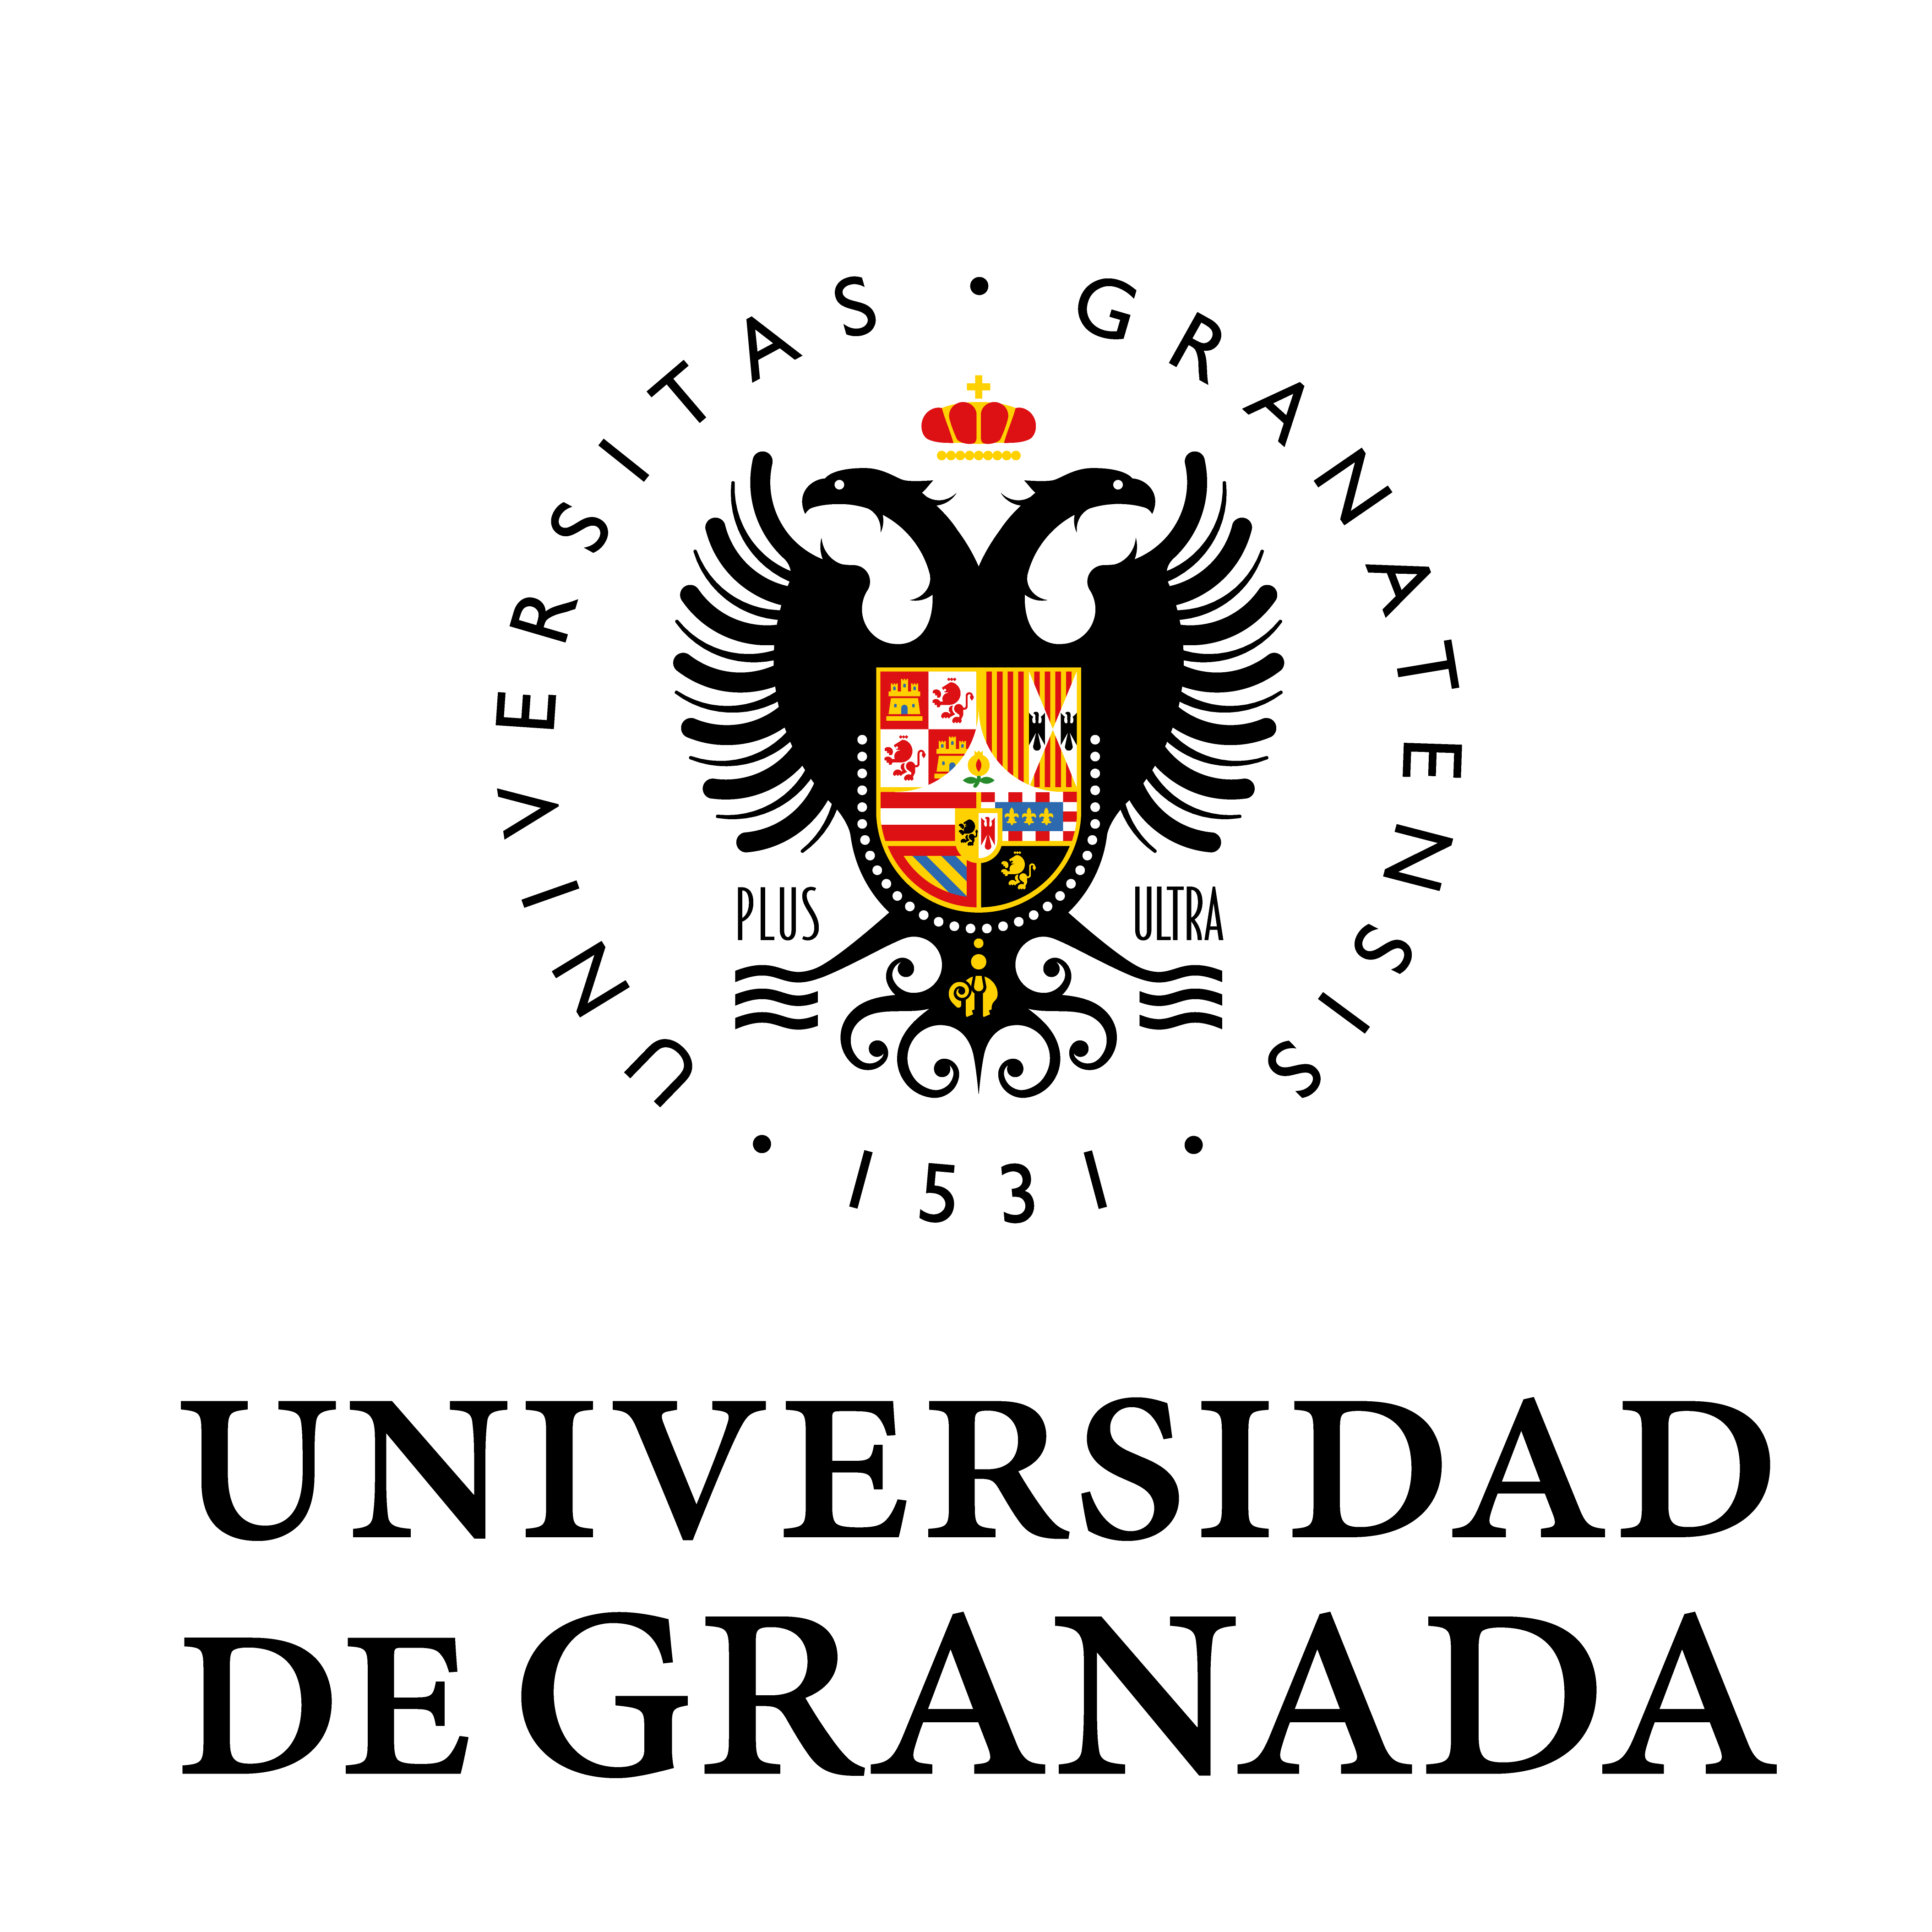
\includegraphics[scale = 0.50]{ugr.png}\\[0.7 cm]
    %\textsc{\LARGE Universidad de Granada}\\[2.0 cm]
    \textsc{\large 4º CSI 2020/21 - Grupo 2}\\[0.5 cm]
    \textsc{\large Grado en Ingeniería Informática}\\[0.5 cm]
    \rule{\linewidth}{0.2 mm} \\[0.2 cm]
    { \huge \bfseries \thetitle}\\
    \rule{\linewidth}{0.2 mm} \\[1 cm]

    \begin{minipage}{0.4\textwidth}
        \begin{flushleft} \large
            \emph{Autor:}\\
            \theauthor\\
			 \emph{DNI:}\\
            77021623-M
            \end{flushleft}
            \end{minipage}~
            \begin{minipage}{0.4\textwidth}
            \begin{flushright} \large
            \emph{Asignatura: \\
            Visión por Computador}   \\
            \emph{Correo:}\\
            advy99@correo.ugr.es
        \end{flushright}
    \end{minipage}\\[0.5cm]

    {\large \thedate}\\[0.5cm]
    %{\url{https://github.com/advy99/AA/}}
    {\doclicenseThis}

    \vfill

\end{titlepage}

%%%%%%%%%%%%%%%%%%%%%%%%%%%%%%%%%%%%%%%%%%%%%%%%%%%%%%%%%%%%%%%%%%%%%%%%%%%%%%%%%%%%%%%%%

\tableofcontents
\pagebreak

%%%%%%%%%%%%%%%%%%%%%%%%%%%%%%%%%%%%%%%%%%%%%%%%%%%%%%%%%%%%%%%%%%%%%%%%%%%%%%%%%%%%%%%%%


\section*{Introducción}

En esta práctica trabajaremos con redes neuronales convolucionales profundas, de cara a obtener experiencia en el diseño y entrenamiento de las mismas utilizando el módulo Keras de Python.

Las redes neuronales convolucionales profundas se componen de operaciones estocásticas, por lo que para obtener los mismos resultados en todos los casos he mantenido la misma semilla en todas las ejecuciones y es la semilla establecida en el código entregado junto a este PDF.

\section{Apartado 1: BaseNet en CIFAR100}

Trabajaremos con el conjunto de datos CIFAR100, que consta de 60.000 imágenes de dimensión 32$\times$32$\times$3 de 100 clases distintas, es decir, 600 imágenes por clase. El conjunto dispone de 50.000 imágenes de entrenamiento y 10.000 imágenes de prueba. Para el desarollo de la práctica solo consideraremos 25 de las 100 clases, por lo tanto el conjunto de entrenamiento tendrá 12500 imágenes y el de prueba 2500. En todos los casos utilizarémos el 10\% del conjunto de entrenamiento como validación.


El modelo inicial que implementaremos será el siguiente:


% Please add the following required packages to your document preamble:
% \usepackage{graphicx}
\begin{table}[H]
\centering
\resizebox{\textwidth}{!}{%
\begin{tabular}{|c|c|c|c|c|}
\hline
\textbf{Número de capa} & \textbf{Tipo de capa} & \textbf{\begin{tabular}[c]{@{}c@{}}Tam. kernel \\ (para convoluciones)\end{tabular}} & \textbf{Tamaño de entrada/salida} & \textbf{\begin{tabular}[c]{@{}c@{}}Canales de entrada/salida \\ para convoluciones)\end{tabular}} \\ \hline
1                       & Conv2D                & 5                                                                                    & 32 | 28                           & 3 | 6                                                                                             \\ \hline
2                       & Relu                  & -                                                                                    & 28 | 28                           & -                                                                                                 \\ \hline
3                       & MaxPooling2D          & 2                                                                                    & 28 | 14                           & -                                                                                                 \\ \hline
4                       & Conv2D                & 5                                                                                    & 14 | 10                           & 6 | 16                                                                                            \\ \hline
5                       & Relu                  & -                                                                                    & 10 | 10                           & -                                                                                                 \\ \hline
6                       & MaxPooling2D          & 2                                                                                    & 10 | 5                            & -                                                                                                 \\ \hline
7                       & Linear                & -                                                                                    & 400 | 50                          & -                                                                                                 \\ \hline
8                       & Relu                  & -                                                                                    & 50 | 50                           & -                                                                                                 \\ \hline
9                       & Linear                & -                                                                                    & 50 | 25                           & -                                                                                                 \\ \hline
10                      & Softmax               & -                                                                                    & 25 | 25                           & -                                                                                                 \\ \hline
\end{tabular}%
}
\end{table}


\subsection{Implementación del modelo: Hiperparámetros y función de cada capa}

Para implementar el modelo utilizaremos la clase \texttt{Sequential} del módulo de Python \texttt{keras.models}, que nos permite agrupar una serie de capas de una red que finalmente conformarán un objeto de la clase \texttt{Model}.

En este modelo encontramos distintos tipos de capas:

\begin{itemize}
	\item Conv2D\cite{conv2d} : Capa cuya función es aplicar una convolución 2D a la entrada.
	\item Relu\cite{relu} : Capa que implementa la función de activación ReLu, vista en teoría.
	\item MaxPooling2D\cite{maxpooling2d} : Implementa la operación de max pooling para datos 2D. Reduce la muestra del input en el valor máximo dado por \texttt{pool\_size} en cada eje.
	\item Linear : Implementada utilizando la capa \texttt{Dense}\cite{dense} de Keras, se trata de una capa densa totalmente conectada.
	\item Softmax\cite{softmax}: Capa para trasformar la salida en la probabilidad de que pertenezca de pertenecer a cada clase
\end{itemize}

Tras esta simple introducción, pasaré a comentar detalladamente los hiperparámetros de cada capa utilizada:

\subsubsection{Capa Conv2D}

En esta capa encontraremos distintos hiperparámetros, principalmente para controlar el tamaño de la máscara, la dimensionalidad de la salida, y otras especificaciones sobre las convoluciones 2D que vimos en la práctica 1. Los más interesantes son:

\begin{itemize}
	\item \texttt{filters}: Dimensionalidad de la salida, es decir, número de filtros de salida en la convolución.
	\item \texttt{kernel\_size}: Tamaño del kernel 2D a aplicar.
	\item \texttt{strides}: Desplazamiento con que aplicar la convolución, por defecto (1,1) ya que se aplicará a toda la entrada.
	\item \texttt{padding}: Relleno al aplicar la convolución, de cara a poder aplicarla a los bordes de la matriz de entrada.
	\item \texttt{activation}: Aplicar una función de activación al final de la operación.

\end{itemize}

En nuestro caso, el valor de \texttt{filters} tendrá el valor de los canales de salida dados en el modelo, \texttt{kernel\_size} tendrá el valor dado en la tabla del modelo, \texttt{strides} utilizaremos el valor por defecto de cara a aplicar la operación a toda la entrada, \texttt{padding} tomará el valor de \texttt{valid} de cara a no aplicar este relleno, y por último, \texttt{activation} no lo utilizaré, ya que he preferido añadir una capa propia de activación. El resultado es equivalente, pero me resulta más cómodo para realizar una clara distinción de que se tratan de operaciones distintas.

\subsubsection{Capa activación ReLu}

Utilizaremos la capa \texttt{Activation} de Keras, que como único parámetro tiene el tipo de activación. En este caso, como nos pide el ejercicio, utilizaremos como función de activación \texttt{relu}. Esta cápa se encargará de decidir si una neurona es activada o no, calculando el peso de esta y teniendo en cuenta el sesgo que podría añadir. El objetivo de este tipo de capas son introducir no linearidad en el modelo.

\subsubsection{Capa MaxPooling2D}

Tiene como objetivo reducir la dimensionalidad de la entrada.

Aunque comparte los parámetros de \texttt{strides} y \texttt{padding} con la capa Conv2D, en nuestro caso el parámetro que nos interesa será \texttt{pool\_size}, este parámetro indicará el factor de reducción de la entrada. De esta forma, como vemos en la tabla del modelo, al aplicar un factor de escala de dos, reduciremos el tamaño de la entrada a la mitad.


\subsubsection{Capa Dense}

Esta capa se trata de una capa de neuronas totalmente conectadas. En esta operación simplemente utilizaremos el parámetro \texttt{units}, con el que indicaremos el número de neuronas de la capa. El tamaño de salida de esta capa coincidirá con el parámetro \texttt{units}.


\subsubsection{Capa Flatten}


Una observación es que vemos como justo antes de aplicar la capa \texttt{Dense} por primera vez en nuestro modelo, pasamos a tener una salida de tamaño cinco, y la entrada a esta capa será de cuatrocientos. Esto es debido a que utilizaremos una capa \texttt{Flatten}\cite{flatten} que reducirá la entrada como un vector 1D, de forma que la capa de tamaño cinco, al tener dieciséis canales, tendrá tamaño cuatrocientos.


\subsubsection{Implementación del modelo}

El modelo por lo tanto se trata de una variable de tipo \texttt{Sequential}, al que con el método \texttt{add} añadiremos las distintas capas con los hiperparámetros dados. Se puede consultar más a fondo en el fichero de Python adjunto a este PDF.


\subsection{Entrenamiento del modelo y valores de accuracy en los conjuntos de validación y test}

Una vez hemos completado nuestro modelo, utilizando un optimizador (en este caso SGD\cite{sgd}), utilizaremos el método \texttt{compile} para compilar el modelo. En este método utilizaremos tres parámetros:

\begin{enumerate}
	\item \texttt{loss}: Tipo de perdida del modelo, en nuestro caso \texttt{keras.losses.categorical\_crossentropy}, ya que trabajamos con un problema multiclase.
	\item \texttt{optimizer}: Optimizador a utilizar, como he comentado, en nuestro caso \texttt{SGD}.
	\item \texttt{metrics}: Métricas para medir el error del modelo. En nuestro caso \texttt{accuracy}.

\end{enumerate}


Una vez compilado el modelo, podemos entrenarlo con la función \texttt{fit}, que cuenta con distintos parámetros, la mayoría de ellos vistos en Aprendizaje Automático, como el número de épocas, el tamaño del batch a utilizar, y el porcentaje de validación del conjunto de entrenamiento. En nuestro caso, utilizaremos un valor de $0.1$ para el porcentaje de validación, como nos indica el enunciado, así como un tamaño de batch de 32, ya que es el valor por defecto y funciona bien.

Tras esto, la evolución del entrenamiento del modelo es la siguiente:


\begin{figure}[H]
  \centering
      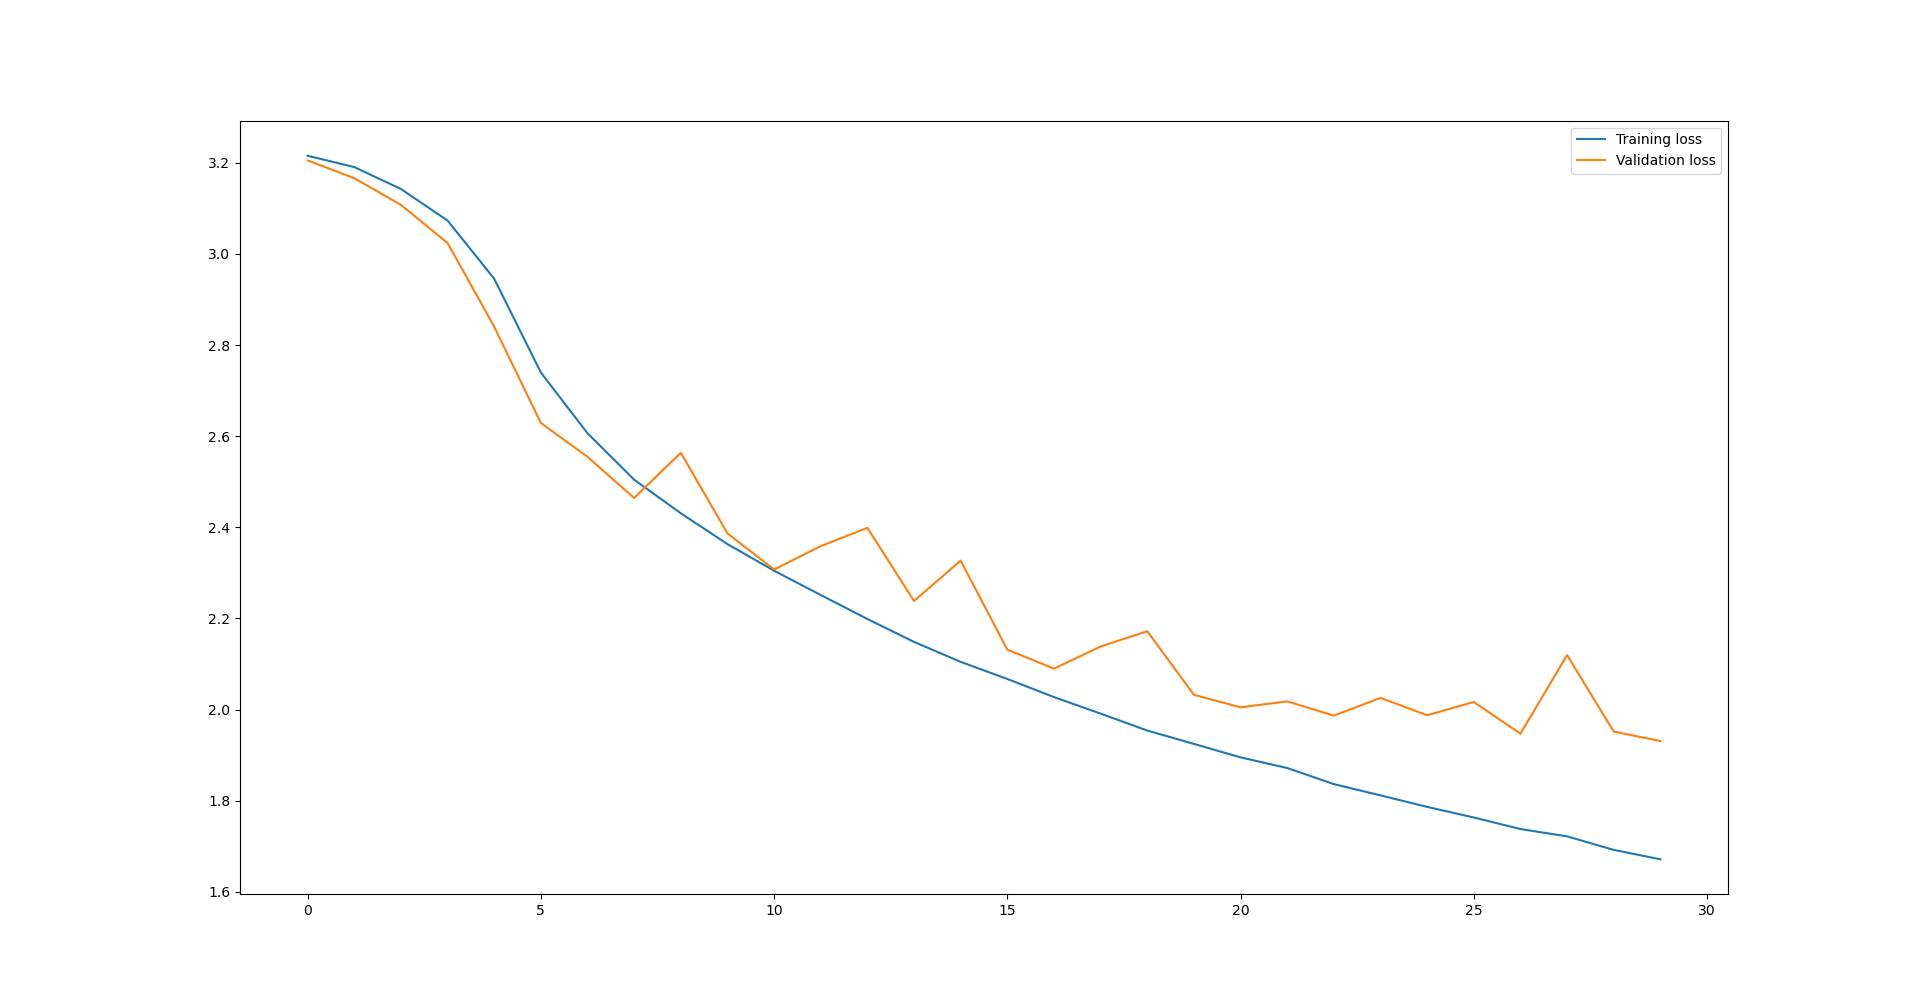
\includegraphics[width=\textwidth]{1-1-1.png}
 		\caption{Perdida en el conjunto de entrenamiento y validación.}
\end{figure}

\begin{figure}[H]
  \centering
      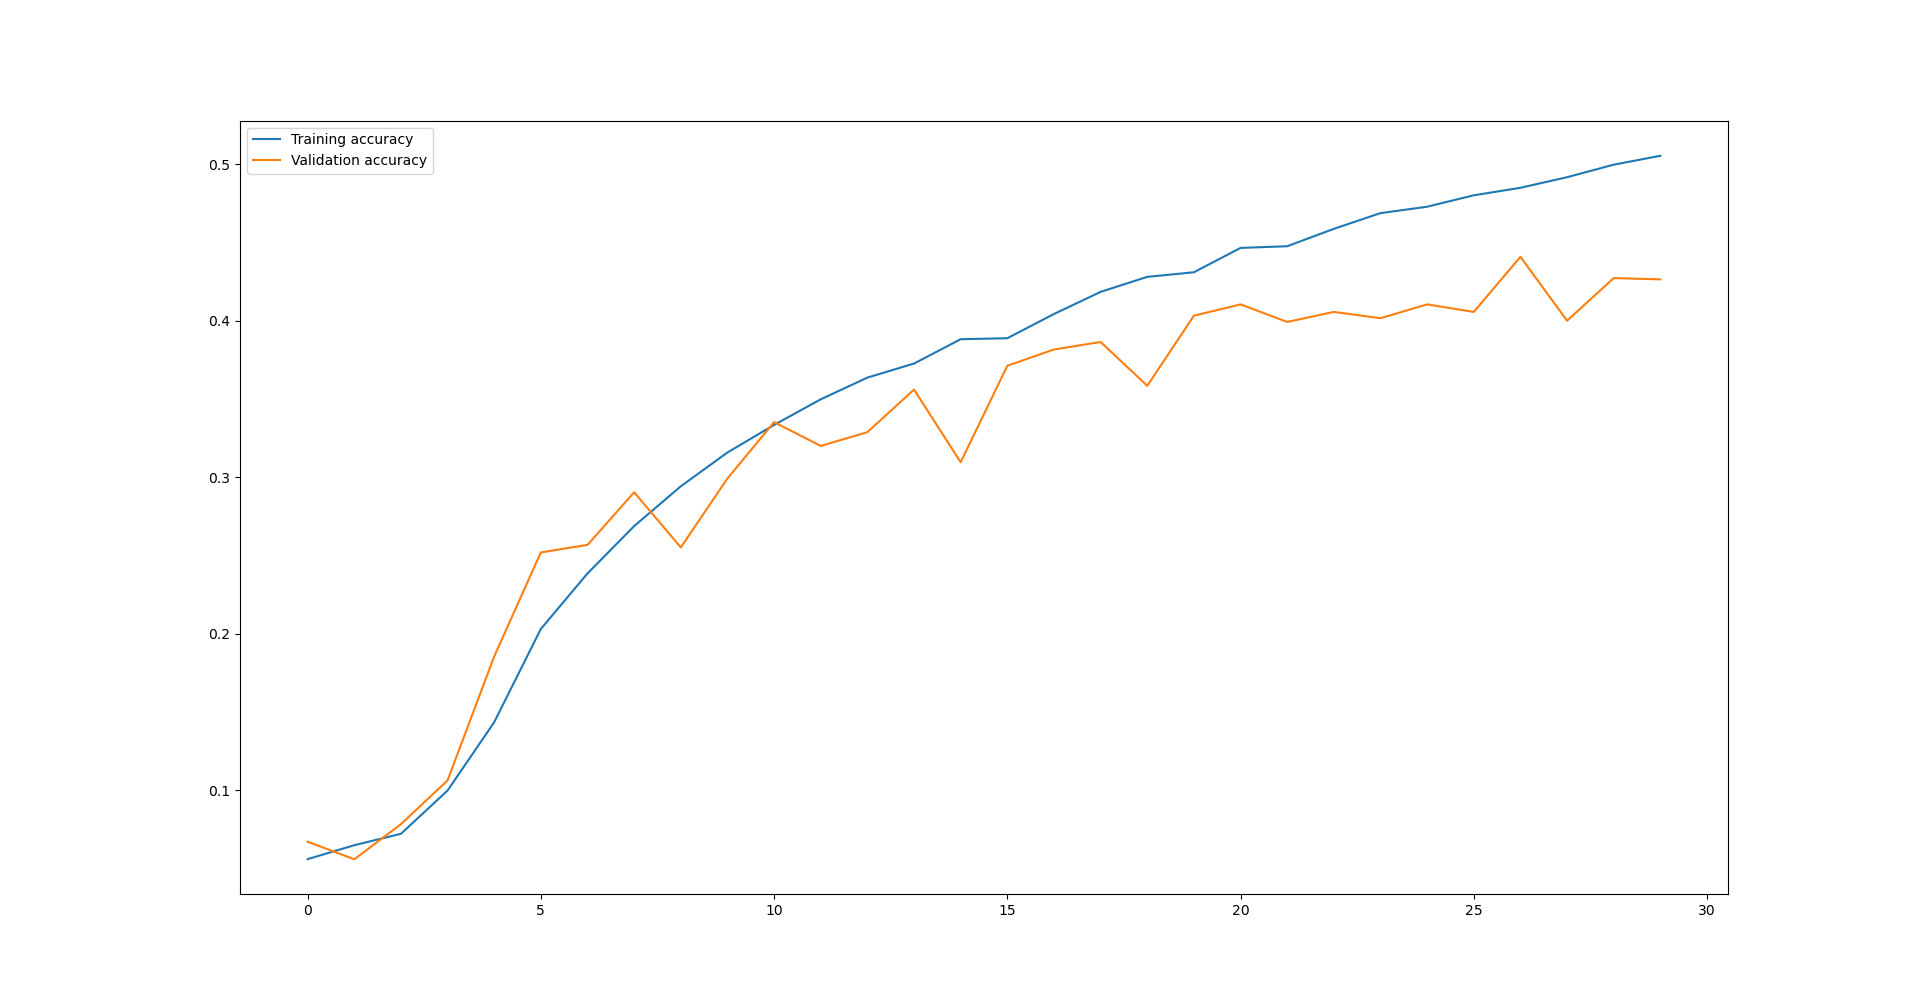
\includegraphics[width=\textwidth]{1-1-2.png}
 		\caption{Valor de precisión en el conjunto de entrenamiento y validación.}
\end{figure}

Observamos como obtenemos un valor de precisión cercano al 42\% en el conjunto de validación, lo que nos lleva a pensar en un resultado mediocre del modelo.

En el conjunto de test conseguimos un valor de precisión similar:

\begin{lstlisting}
Accuracy en el conjunto test: 0.438
\end{lstlisting}

\section{Apartado 2: Mejora del modelo BaseNet}

Hemos visto que el resultado obtenido no es el mejor posible, por lo que en este apartado trataremos de mejorar el modelo. Como se nos comenta en el enunciado, con una buena combinación de capas podemos obtener que el valor de precisión se acerque al 50\%, por este motivo en este apartado aplicaré mejoras en el modelo hasta llegar a ese porcentaje, y las demás mejoras las dejaré para el ejercicio de bonus, que se nos pide seguir mejorando el modelo.


Debido a que las mejoras que he ido probando mejoraban poco a poco el modelo, cada mejora añadida la he mantenido en la siguiente mejora, es decir, por ejemplo, al aplicar normalización, en la mejora de aumento de datos cuenta con el aumento de datos y con la normalización.

\subsection{Normalización de datos}

De cara a obtener un entrenamiento más sencillo y sólido, he utilizado la normalización de datos. Para aplicar esta normalización he utilizado la clase \texttt{ImageDataGenerator}\cite{imagedatagenerator}. Esta clase la utilizaremos a lo largo de todo el apartado ya que nos permite realizar varias de las mejoras propuestas.

Con esta clase conseguiremos, dado una entrada de imágenes, obtener imágenes modificadas a partir de las originales, desde normalización de las imagenes, aumento de las imágenes con zoom, volteados, rotaciones, etc.

En este apartado en concreto usaremos los parámetros \texttt{featurewise\_center}, que estableceremos a \texttt{True}, para hacer que la media de la entrada sea cero, y \texttt{featurewise\_std\_normalization} que también estará a \texttt{True}, para que la desviación típica sea de uno.

De esta forma, declararemos estos generadores de imágenes y al entrenar el modelo, en lugar de utilizar el método \texttt{fit} usaremos el método \texttt{fit\_generator}, al que le podemos pasar una serie de imágenes generadas con el método \texttt{flow} de los generadores de imágenes.

Otra cuestión importante de utilizar estos generadores de datos es que en su declaración debemos especificar el porcentaje a usar de validación, y al aplicar el método \texttt{fit\_generator} para referirnos al conjunto de entrenamiento usaremos el subconjunto de training con el parámetro \texttt{subset} de \texttt{flow}, y para referirnos al conjunto de validación usaremos \texttt{validation\_data} con el \texttt{subset} de \texttt{validation}.

Por último, a la hora de probar el resultado con el conjunto de test, este conjunto tendrá su propio \texttt{ImageDataGenerator}, que normalizará las imágenes, pero no las separará dos conjuntos, uno de ellos para validación.


Tras aplicar este cambio, los resultados son los siguientes:



\begin{figure}[H]
  \centering
      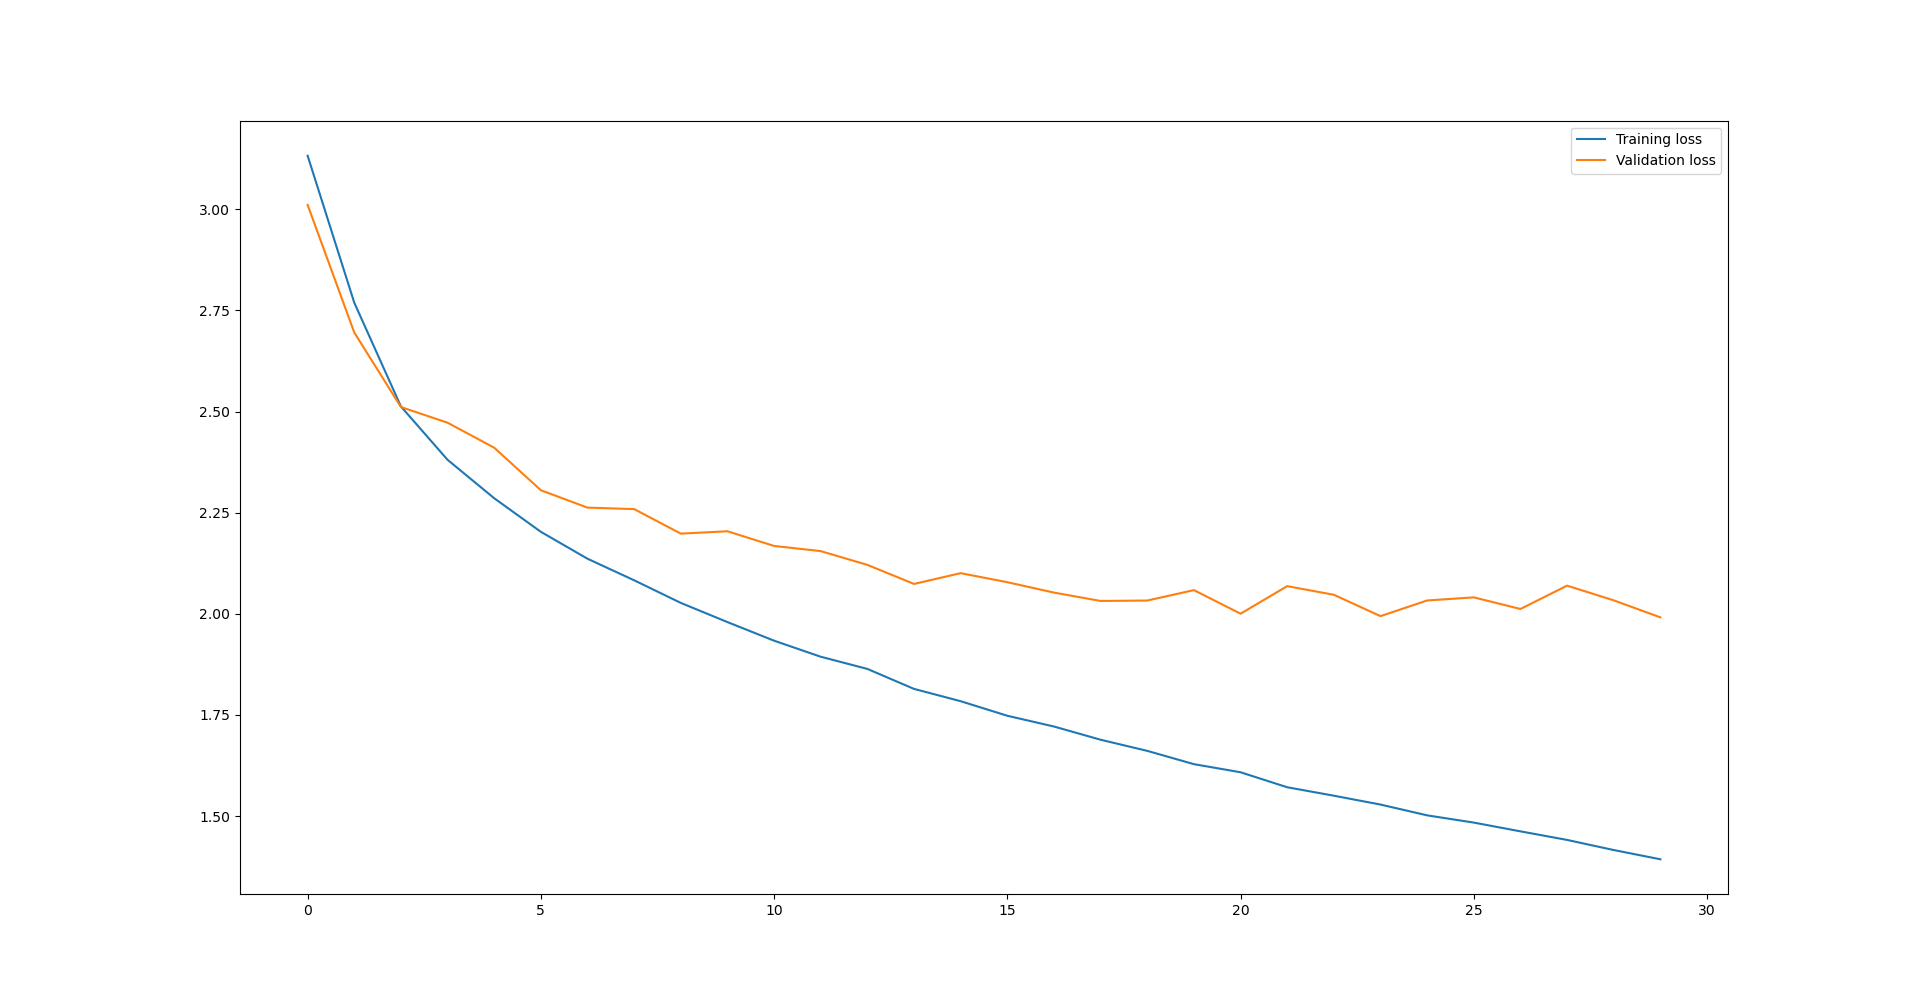
\includegraphics[width=\textwidth]{1-2-norm.png}
 		\caption{Perdida en el conjunto de entrenamiento y validación aplicando normalización de media 0 y varianza 1 a la entrada.}
\end{figure}

\begin{figure}[H]
  \centering
      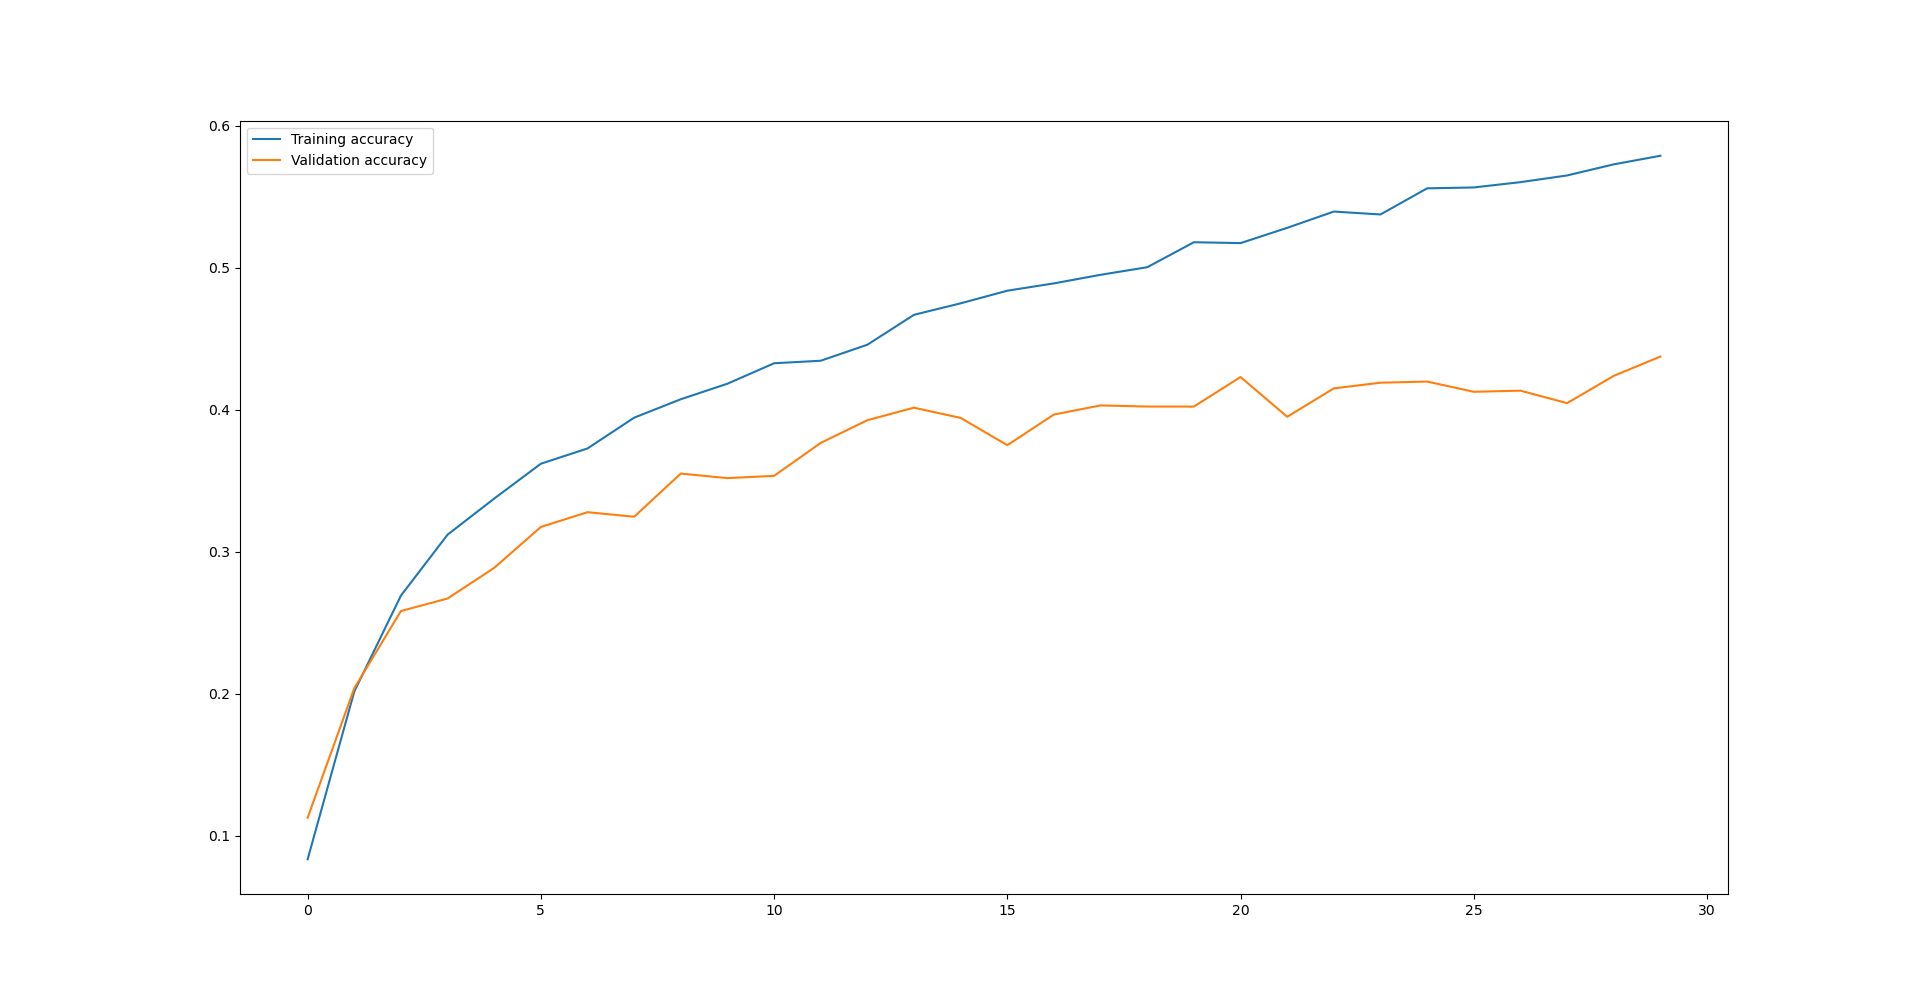
\includegraphics[width=\textwidth]{1-2-norm-2.png}
 		\caption{Valor de precisión en el conjunto de entrenamiento y validación aplicando normalización de media 0 y varianza 1 a la entrada.}
\end{figure}



En el conjunto de test conseguimos el siguiente valor de precisión:

\begin{lstlisting}
Accuracy en el conjunto test con normalización: 0.4524
\end{lstlisting}

Vemos como tanto en el conjunto de validación como en el conjunto de test supone una pequeña mejora.


\subsection{Aumento de datos}

Esta mejora trata de generar más variedad de imágenes del conjunto de entrenamiento dado. En concreto utilizaré el parámetro \texttt{horizontal\_flip} para que además de las imágenes que conformal el conjunto de entrenamiento entrene también con dichas imágenes volteadas de forma horizontal. También probé con \texttt{vertical\_flip}, sin embargo no daba buenos resultados ya que voltear verticalmente las imagenes no aporta gran información, ya que es raro encontrarse imágenes del reves, sin embargo es común encontrar imágenes y escenas simetricas horizontalmente.

Otro de los posibles parámetros es \texttt{zoom\_range}, que genera nuevas imágenes a partir de aplicar zoom a las originales, sin embargo al ser demasiadas imagenes con las que entrenar y que no conseguia un buen ajuste de forma experimental, decidí descartarlo.

Como nos comenta el guión de prácticas, es importante generar tres \texttt{ImageDataGenerator} distintos, uno para el conjunto de entrenamiento, otro para el conjunto de validación y otro para el conjunto de test. Esto se debe a que el conjunto de entrenamiento y validación tienen que conformarlo con cierto porcentaje concreto de imágenes, sin embargo no podemos utilizar el parámetro \texttt{subset} utilizado en la mejora anterior, ya que es importante que solo se valide con las imágenes originales, no con las generadas por el volteado. Los motivos de usar un \texttt{ImageDataGenerator} para el conjunto de test son las mismas que en el apartado anterior.

Esta mejora también incluye la normalización de datos explicada en el apartado anterior.

Los resultados son los siguientes:

\begin{figure}[H]
  \centering
      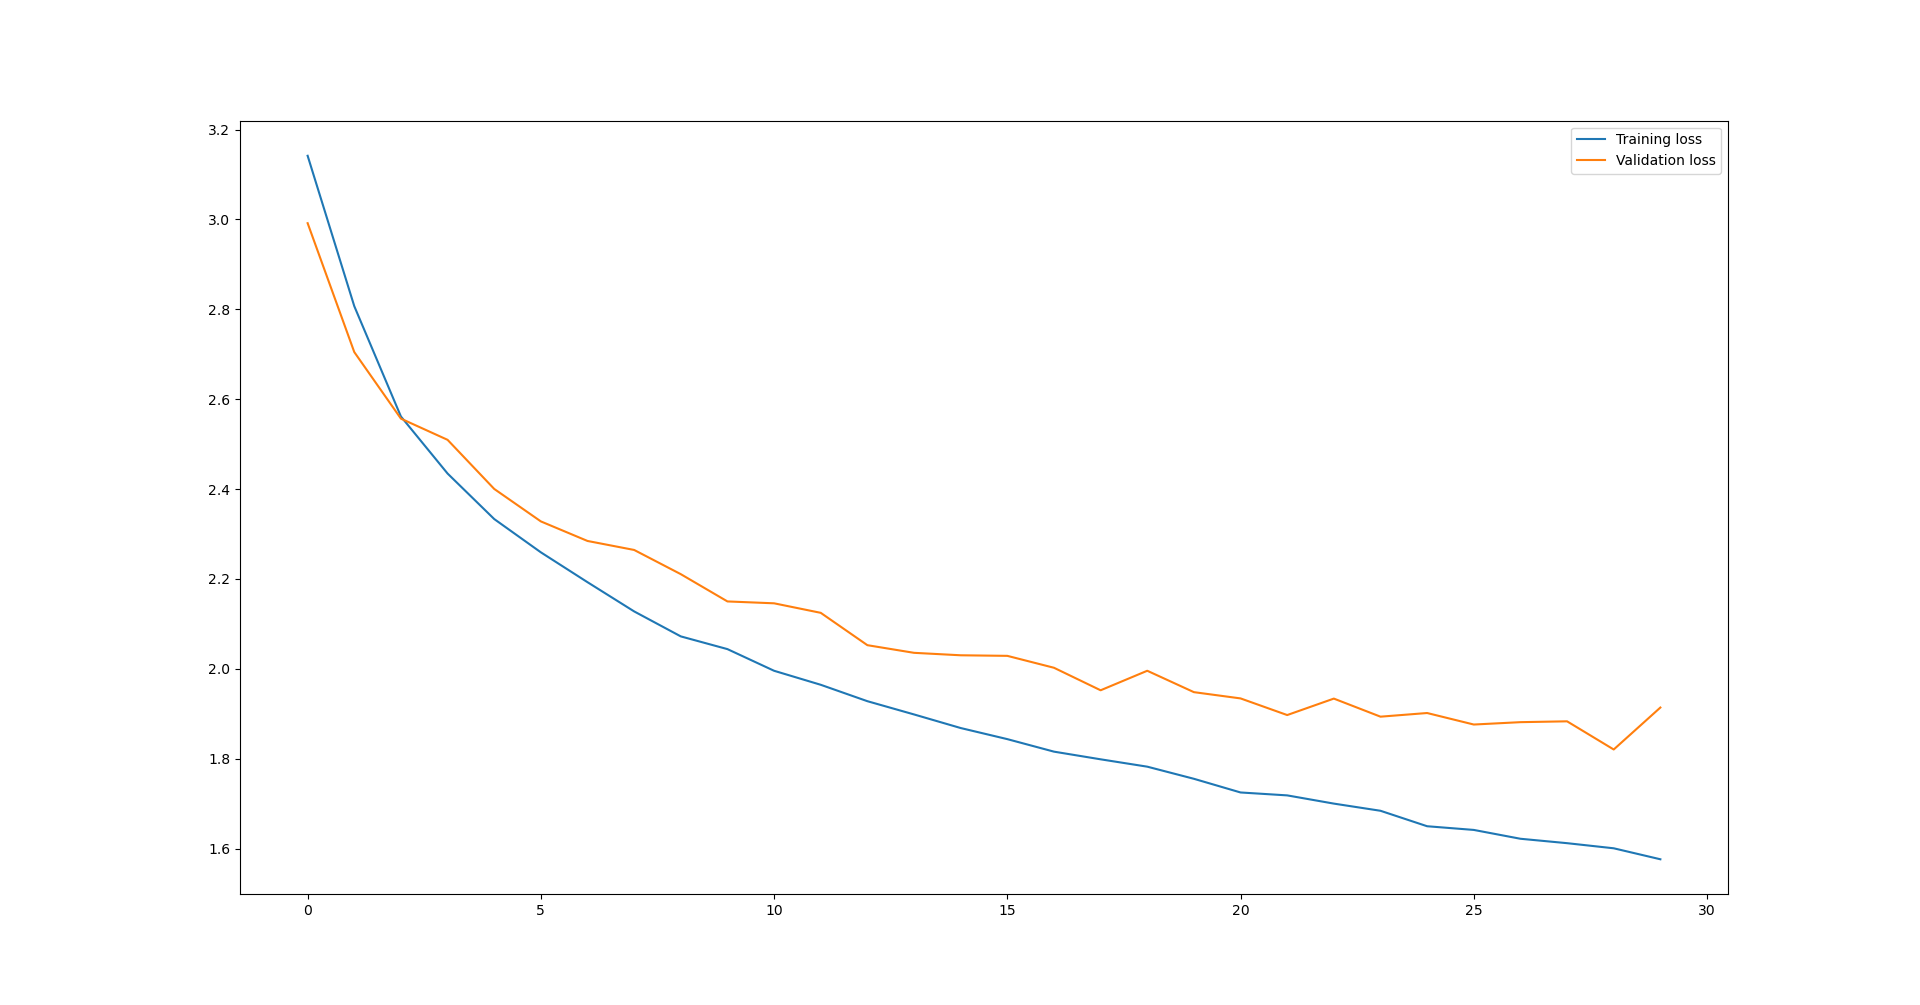
\includegraphics[width=\textwidth]{1-2-aumento.png}
 		\caption{Perdida en el conjunto de entrenamiento y validación aplicando normalización de media 0 y varianza 1 y aumento de datos a la entrada.}
\end{figure}

\begin{figure}[H]
  \centering
      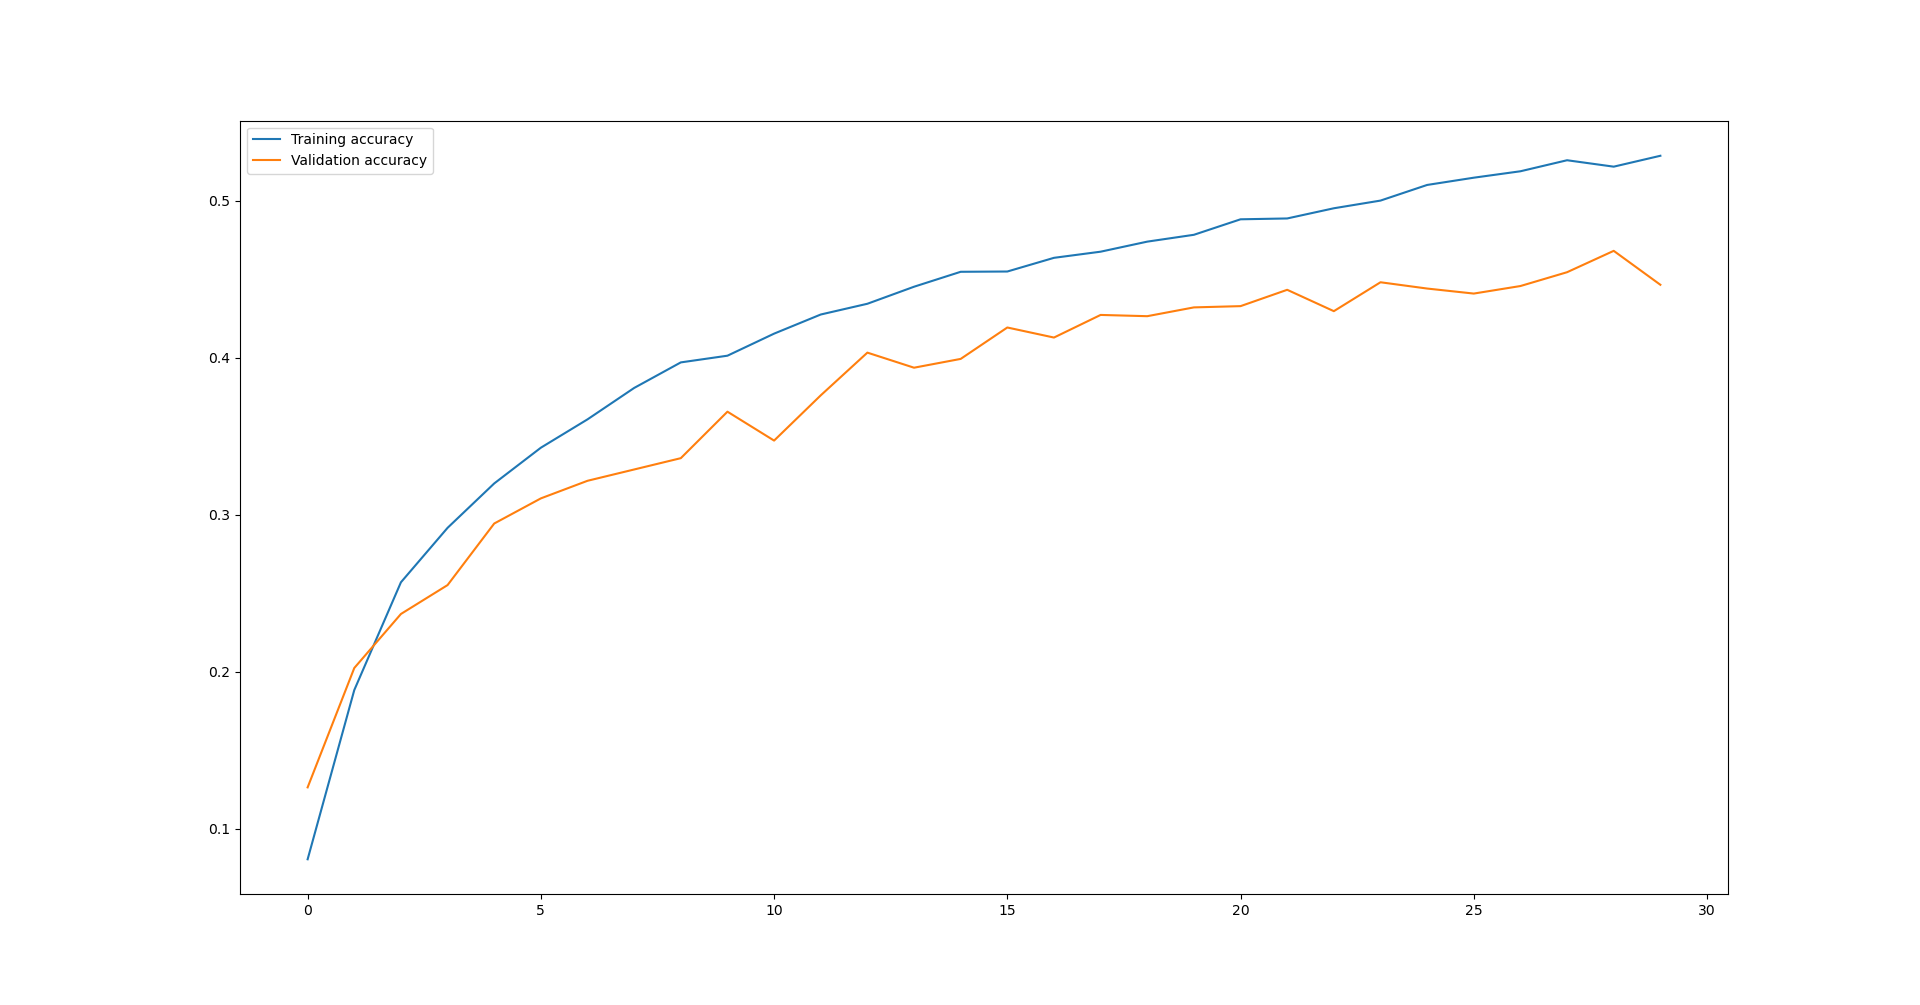
\includegraphics[width=\textwidth]{1-2-aumento-2.png}
 		\caption{Valor de precisión en el conjunto de entrenamiento y validación aplicando normalización de media 0 y varianza 1 y aumento de datos a la entrada.}
\end{figure}



En el conjunto de test conseguimos el siguiente valor de precisión:

\begin{lstlisting}
Accuracy en el conjunto test con normalizacion y aumento: 0.4764
\end{lstlisting}

En este caso también se mejora el modelo, acercandose al objetivo del 50\% de precisión.

\subsection{Normalización con BatchNormalization}

En esta mejora introduciremos nuevas capas de BatchNormalization\cite{batchnormalization} entre las capas de convolución y las capas de activación ReLu.

Estas capas aplicarán una normalización a los datos que mantiene la media de los datos cercana a cero y la desviación típica cercana a uno. Por este motivo la aplicaremos despues de aplicar una convolución, ya que es la operación que modifica los valores de la entrada. De cara a que el comportamiento sea aún mejor utilizaremos el parámetro \texttt{renorm} de esta capa, ya que ayuda a la forma en la que se trabaja con los minibatch en la normalización\cite{renorm}.


Con estas modificaciones el modelo quedaría de la siguiente forma:

% Please add the following required packages to your document preamble:
% \usepackage{graphicx}
\begin{table}[H]
\centering
\resizebox{\textwidth}{!}{%
\begin{tabular}{|c|c|c|c|c|}
\hline
\textbf{Número de capa} & \textbf{Tipo de capa} & \textbf{\begin{tabular}[c]{@{}c@{}}Tam. kernel \\ (para convoluciones)\end{tabular}} & \textbf{Tamaño de entrada/salida} & \textbf{\begin{tabular}[c]{@{}c@{}}Canales de entrada/salida \\ para convoluciones)\end{tabular}} \\ \hline
1                       & Conv2D                & 5                                                                                    & 32 | 28                           & 3 | 6                                                                                             \\ \hline
2                       & BatchNormalization    & -                                                                                    & 28 | 28                           & -                                                                                                 \\ \hline
3                       & Relu                  & -                                                                                    & 28 | 28                           & -                                                                                                 \\ \hline
4                       & MaxPooling2D          & 2                                                                                    & 28 | 14                           & -                                                                                                 \\ \hline
5                       & Conv2D                & 5                                                                                    & 14 | 10                           & 6 | 16                                                                                            \\ \hline
6                       & BatchNormalization    & -                                                                                    & 10 | 10                           & -                                                                                                 \\ \hline
7                       & Relu                  & -                                                                                    & 10 | 10                           & -                                                                                                 \\ \hline
8                       & MaxPooling2D          & 2                                                                                    & 10 | 5                            & -                                                                                                 \\ \hline
9                       & Linear                & -                                                                                    & 400 | 50                          & -                                                                                                 \\ \hline
10                      & BatchNormalization    & -                                                                                    & 50 | 50                           & -                                                                                                 \\ \hline
11                      & Relu                  & -                                                                                    & 50 | 50                           & -                                                                                                 \\ \hline
12                      & Linear                & -                                                                                    & 50 | 25                           & -                                                                                                 \\ \hline
13                      & Softmax               & -                                                                                    & 25 | 25                           & -                                                                                                 \\ \hline
\end{tabular}%
}
\end{table}


Y los resultados obtenidos son los siguientes:

\begin{figure}[H]
  \centering
      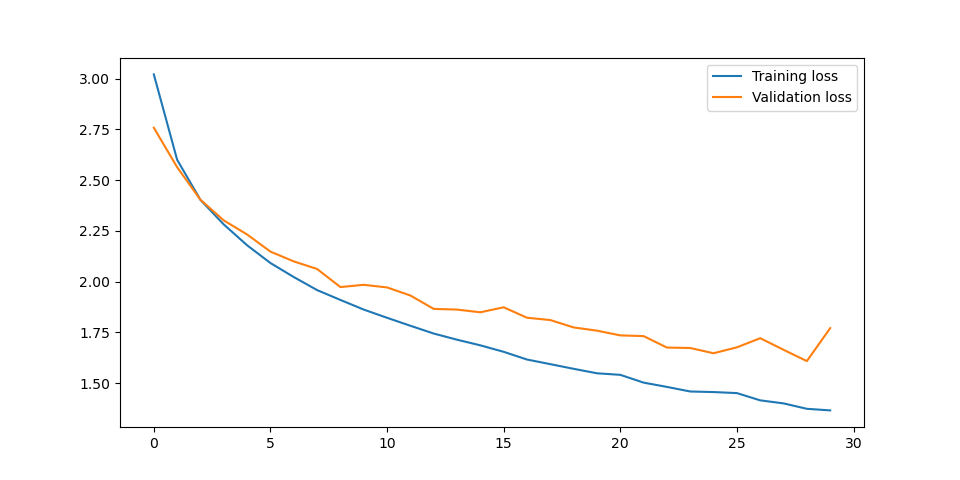
\includegraphics[width=\textwidth]{1-2-batch.png}
 		\caption{Perdida en el conjunto de entrenamiento y validación aplicando normalización de media 0 y varianza 1, aumento de datos y BatchNormalization.}
\end{figure}

\begin{figure}[H]
  \centering
      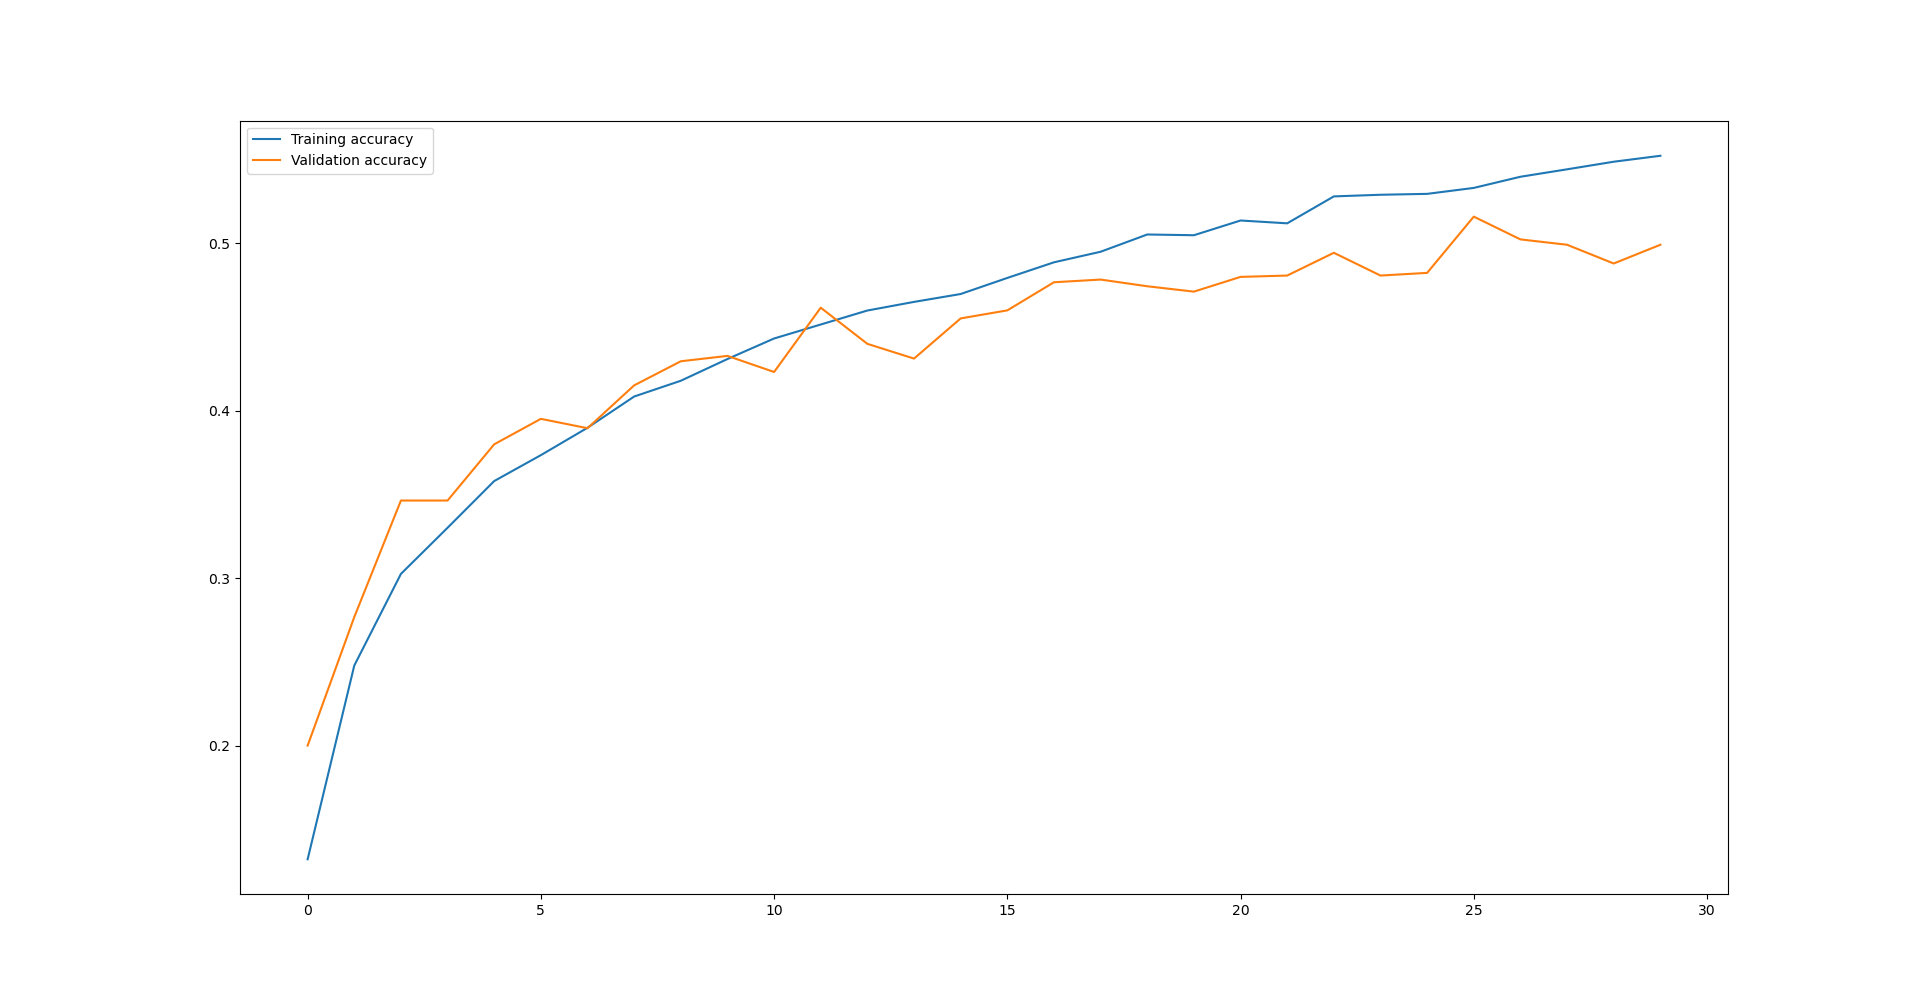
\includegraphics[width=\textwidth]{1-2-batch-2.png}
 		\caption{Valor de precisión en el conjunto de entrenamiento y validación aplicando normalización de media 0 y varianza 1, aumento de datos y BatchNormalization.}
\end{figure}



En el conjunto de test conseguimos el siguiente valor de precisión:

\begin{lstlisting}
Accuracy en el conjunto test con normalizacion, aumento y batch normalization: 0.5064
\end{lstlisting}

Vemos como con esta mejora ya conseguimos superar el 50\% de precisión pedido por este ejercicio.





\subsection{Regularización con Dropout}

Por último, la mejora final que he aplicado (fuera del ejercicio bonus) es la regularización con capas \texttt{Dropout}\cite{dropout}. Esta capa nos ayudará a prevenir el sobreajuste, estableciendo un porcentaje aleatorio dado de entradas a cero.

Estas capas las utilizaré justo antes de una convolución o una capa totalmente conectada, y debido a que el tamaño de la red no es muy grande y tenemos unos datos asequibles, el porcentaje aleatorio utilizado será bajo, de entre $5$ y $10$ \%. De forma empírica he comprobado que si utilizo valores más altos empeoran los resultados, debido a que la perdida de información es demasiado sustancial.

El modelo final sería el siguiente:

% Please add the following required packages to your document preamble:
% \usepackage{graphicx}
\begin{table}[H]
\centering
\resizebox{\textwidth}{!}{%
\begin{tabular}{|c|c|c|c|c|}
\hline
\textbf{Número de capa} & \textbf{Tipo de capa} & \textbf{\begin{tabular}[c]{@{}c@{}}Tam. kernel \\ (para convoluciones)\end{tabular}} & \textbf{Tamaño de entrada/salida} & \textbf{\begin{tabular}[c]{@{}c@{}}Canales de entrada/salida \\ para convoluciones)\end{tabular}} \\ \hline
1                       & Conv2D                & 5                                                                                    & 32 | 28                           & 3 | 6                                                                                             \\ \hline
2                       & BatchNormalization    & -                                                                                    & 28 | 28                           & -                                                                                                 \\ \hline
3                       & Relu                  & -                                                                                    & 28 | 28                           & -                                                                                                 \\ \hline
4                       & MaxPooling2D          & 2                                                                                    & 28 | 14                           & -                                                                                                 \\ \hline
5                       & Dropout               & -                                                                                    & 14 | 14                           & -                                                                                                 \\ \hline
6                       & Conv2D                & 5                                                                                    & 14 | 10                           & 6 | 16                                                                                            \\ \hline
7                       & BatchNormalization    & -                                                                                    & 10 | 10                           & -                                                                                                 \\ \hline
8                       & Relu                  & -                                                                                    & 10 | 10                           & -                                                                                                 \\ \hline
9                       & MaxPooling2D          & 2                                                                                    & 10 | 5                            & -                                                                                                 \\ \hline
10                      & Dropout               & -                                                                                    & 10 | 5                            & -                                                                                                 \\ \hline
11                      & Linear                & -                                                                                    & 400 | 50                          & -                                                                                                 \\ \hline
12                      & BatchNormalization    & -                                                                                    & 50 | 50                           & -                                                                                                 \\ \hline
13                      & Relu                  & -                                                                                    & 50 | 50                           & -                                                                                                 \\ \hline
14                      & Dropout               & -                                                                                    & 50 | 50                           & -                                                                                                 \\ \hline
15                      & Linear                & -                                                                                    & 50 | 25                           & -                                                                                                 \\ \hline
16                      & Softmax               & -                                                                                    & 25 | 25                           & -                                                                                                 \\ \hline
\end{tabular}%
}
\end{table}

Y los resultados obtenidos son los siguientes:

\begin{figure}[H]
  \centering
      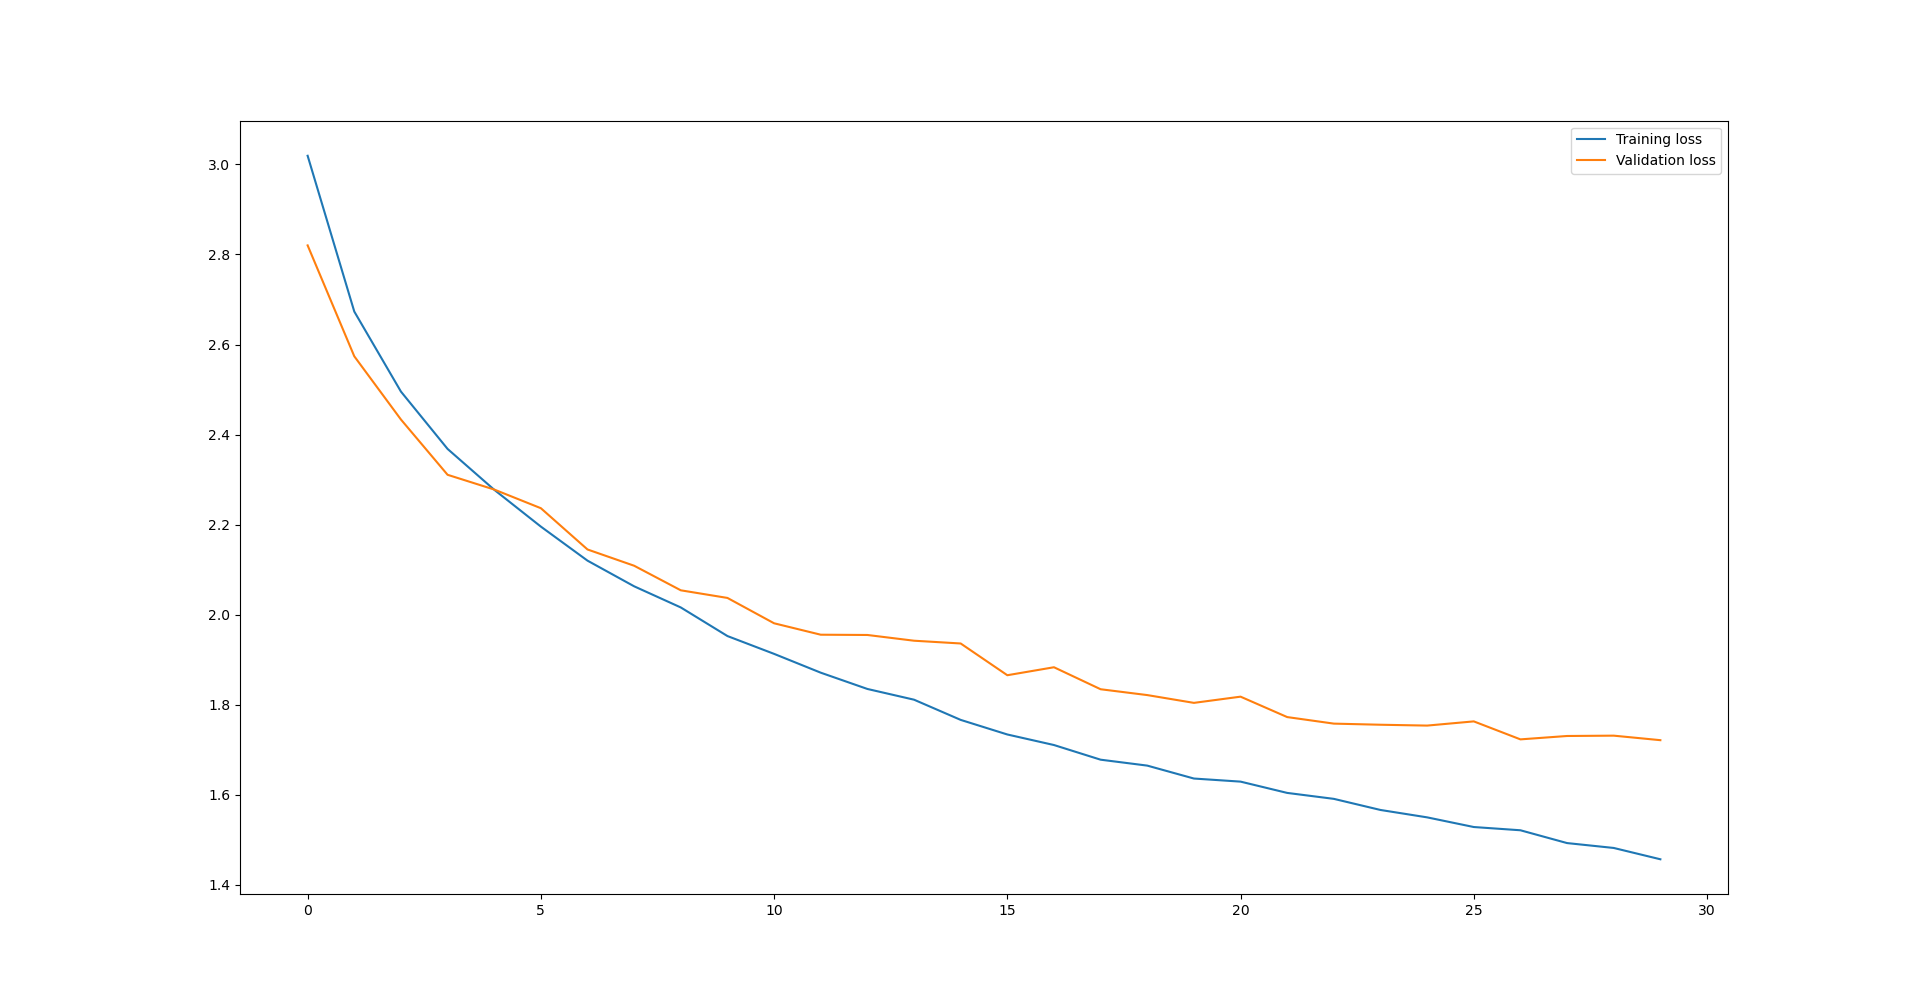
\includegraphics[width=\textwidth]{1-2-dropout.png}
 		\caption{Perdida en el conjunto de entrenamiento y validación aplicando normalización de media 0 y varianza 1, aumento de datos, BatchNormalization y Dropout.}
\end{figure}

\begin{figure}[H]
  \centering
      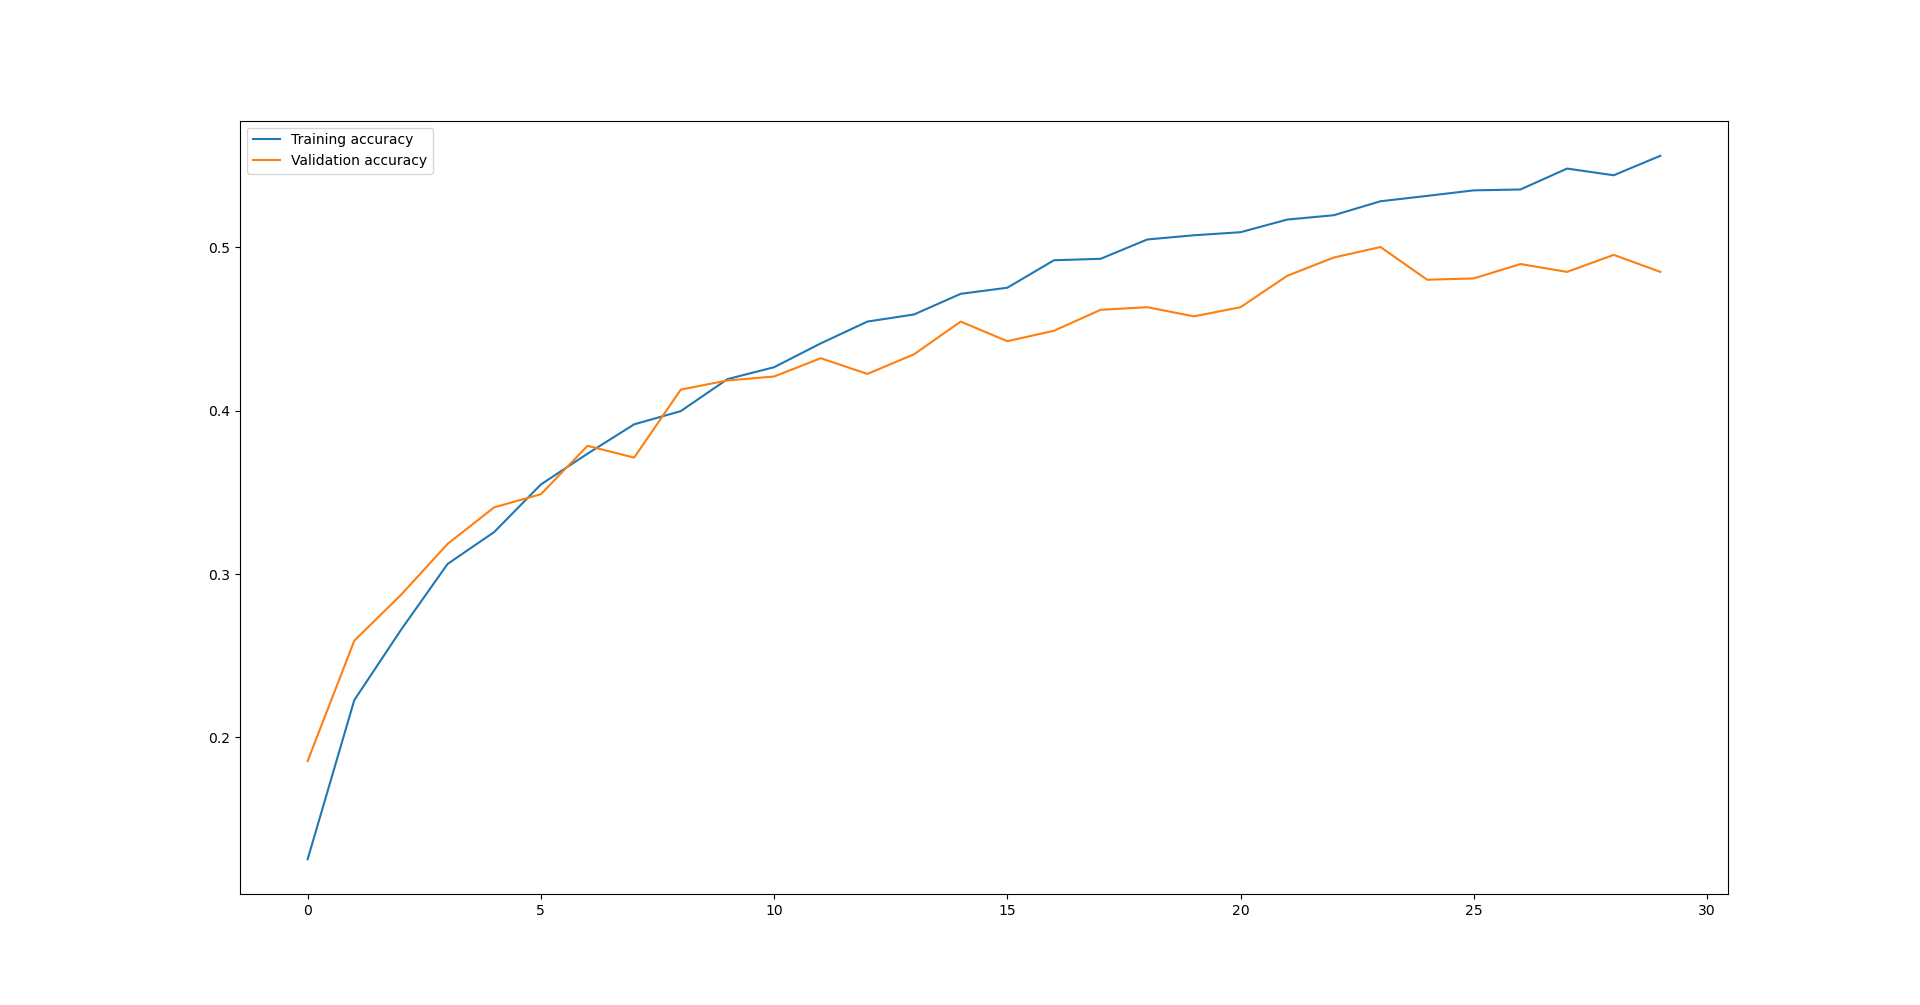
\includegraphics[width=\textwidth]{1-2-dropout-2.png}
 		\caption{Valor de precisión en el conjunto de entrenamiento y validación aplicando normalización de media 0 y varianza 1, aumento de datos, BatchNormalization y Dropout.}
\end{figure}



En el conjunto de test conseguimos el siguiente valor de precisión:

\begin{lstlisting}
Accuracy en el conjunto test con normalizacion, aumento, batch normalization y dropout: 0.5172
\end{lstlisting}

En este caso vemos como mantiene el resultado, sin embargo en las gráficas vemos como la diferencia entre los valores de training y validación en este caso apenas son notables comparados con los casos anteriores, por lo que evitamos el sobreajuste que nos hacía estancarnos anteriormente.

Aun así, se logra superar lo pedido en el ejercicio, ya que se nos decía que con una buena mejora conseguiríamos un modelo que se acerque al 50\% de precisión, y el modelo propuesta la supera.



\newpage






\section{Apartado 3: Transferencia de modelos y ajuste fino con ResNet50 para la base de datos Caltech-UCSD}

Para este apartado utilizaremos los datos de Caltech-UCSD-CUB-200\cite{cub200}, que consta de 6033 imágenes de 200 especies de pájaros, por lo que tendremos 200 clases, 3000 imágenes en el conjunto de entrenamiento y 3033 en el conjunto de prueba, de nuevo utilizaremos el 10\% del conjunto de entrenamiento como validación.

En lugar de crear un modelo desde cero, trabajaremos con una red neuronal convolucional profunda pre-entrenada con ImageNet y disponible en el módulo de Keras, ResNet50\cite{resnet50}.


\subsection{Prueba de modificación de la red pre-entrenada sustitución de la última capa FC y la salida por una red propia}

En este primer apartado se nos pide eliminar la salida y la última capa de ResNet50, y sustituirlas por una nuevas capas entrenadas, de forma que solo entrenemos las dos nuevas capas añadidas.

Para realizar este apartado he utilizado el parámetro \texttt{include\_top} de ResNet50 en Keras, de forma que si esta a false, elimina las capas que nos pide el ejercicio. También estableceremos \texttt{pooling} a \texttt{avg}, ya que en el siguiente apartado nos pide comparar sin esta capa.

También utilizaremos el atributo \texttt{trainable} del modelo pre-entrenado, lo estableceremos a falso, de forma que no se entrene la parte original.

Declararemos un ImageDataGenerator con el parámetro \texttt{preprocessing\_function} con el valor de \texttt{preprocess\_input} de ResNet50, de forma que todas las imagenes de este generador de datos se les aplique las transformaciones de ResNet50.

Tras esto, simplemente obtenemos las caracteristicas tanto para el conjunto de entrenamiento como para test, obtenidas de dicho modelo (sin las dos últimas capas) con el método \texttt{predict\_generator}.


Declararemos un nuevo modelo con \texttt{Sequential} de únicamente dos capas \texttt{Dense}, es decir, FC, como se nos pide, en la que la primera capa tendrá la forma de las caracteristicas obtenidas por \texttt{predict\_generator} y la segunda capa tendrá una salida de tamaño 200 y una activación softmax para devolver la salida, como en el modelo BaseNet, pero en lugar de tener las 25 posibles clases en este problema tenemos 200.

Tras realizar esto, entrenamos el modelo con las caracteristicas obtenidas de la red pre-entrenada, que nuestra red más pequeña tendrá de entrada. El resultado de este entrenamiento es el siguiente:



\begin{figure}[H]
  \centering
      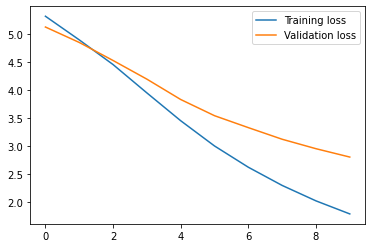
\includegraphics[width=\textwidth]{3-1-a-1.png}
 		\caption{Perdida en el conjunto de entrenamiento y validación entrenando unicamente las dos últimas capas propias.}
\end{figure}

\begin{figure}[H]
  \centering
      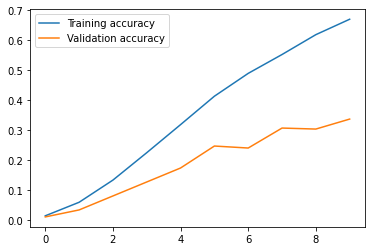
\includegraphics[width=\textwidth]{3-1-a-2.png}
 		\caption{Valor de precisión en el conjunto de entrenamiento y validación entrenando unicamente las dos últimas capas propias.}
\end{figure}



En el conjunto de test conseguimos el siguiente valor de precisión:

\begin{lstlisting}
El accuracy en test es de: 0.30201121002307946
\end{lstlisting}




\subsection{Eliminar las dos últimas capas, además de la capa AveragePooling, añadir nuevas capas para realizar pruebas}

En este caso he procedido como en el caso anterior, solo que al obtener el modelo ResNet50 he establecido el parámetro \texttt{pooling} a \texttt{None} para que no añada la última capa de AveragePooling.

Al nuevo modelo, en lugar de ser dos capas FC como el caso anterior, se trata de un \texttt{Dropout}, seguido de una capa \texttt{Conv2D}, y tras eso una capa \texttt{BatchNormalization} y una capa \texttt{Activation} de tipo ReLu. Finalmente he añadido una capa \texttt{GlobalAveragePooling} de cara a obtener la forma de la salida necesaria para la última capa FC, al igual que estaba en el modelo original, y he dado la salida con una capa FC con una activación softmax.

En resumen, el eliminar la capa de AveragePooling nos ha permitido introducir más capas en el modelo.


\begin{figure}[H]
  \centering
      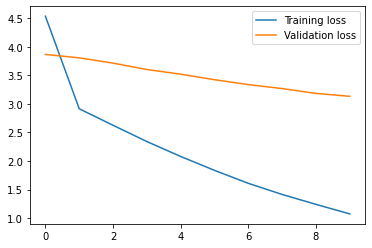
\includegraphics[width=\textwidth]{3-1-b-1.png}
 		\caption{Perdida en el conjunto de entrenamiento y validación entrenando unicamente el nuevo modelo añadido.}
\end{figure}

\begin{figure}[H]
  \centering
      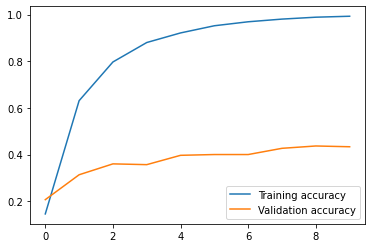
\includegraphics[width=\textwidth]{3-1-b-2.png}
 		\caption{Valor de precisión en el conjunto de entrenamiento y validación entrenando unicamente el nuevo modelo añadido.}
\end{figure}



En el conjunto de test conseguimos el siguiente valor de precisión:

\begin{lstlisting}
El accuracy en test para el apartado B es de: 0.43158588855918234
\end{lstlisting}

Vemos como en este caso mejoramos el resultado del apartado A, y es que como era de esperar, el añadir una convolución y ajustarla a los datos de entrada permite que la red se ajuste mejor a la red del apartado A, en la que solo ajustaba la capa de salida.


\subsection{Ajuste fino de ResNet50}

El ajuste fino\cite{finetuningkeras} se trata de, utilizando redes neuronales convolucionales profundas pre-entrenadas, fijar las capas de la red neuronal convolucional pre-entrenada, y entrenar únicamente las nuevas capas que todavía no están entrenadas, tras esto, desfijar las capas de la red pre-entrenada y entrenar toda la red completa (pre-entrenada y nuevas capas añadidas). Esto nos mejorará los resultados, ya que permite entrenar las capas nuevas de la red, y cuando estas ya estén entrenadas, entrenar todo el conjunto, de forma que las nuevas capas no afecten de forma negativa a la red pre-entrenada, al todavía no estar preparadas y con unos pesos adecuados.

Para desarrollar he consultado varios artículos\cite{finetuningkeras}\cite{finetuning}. He realizado los pasos anteriores, pero en lugar de dar como entrada a la nueva red las caracteristicas obtenidas con ResNet50, he creado la nueva red añadiendo capas a la red de ResNet50, gracias al atributo \texttt{output} de la clase \texttt{Model}. Cabe destacar que antes de hacer esto he fijado las capas de la ResNet50 para que no sean entrenables.

Con todas esas capas, he creado el modelo y lo he entrenado, una vez está entrenado, se han vuelto a hacer entrenables las capas de ResNet50 y recompilado el modelo con las nuevas capas y sus pesos entrenados, de forma que se ha entrenado todo el conjunto de la red.

El resultado entrenando solo las nuevas capas es el siguiente:


\begin{figure}[H]
  \centering
      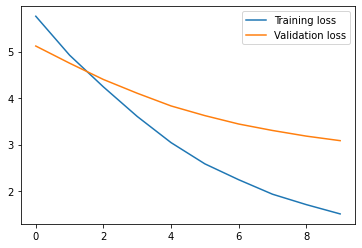
\includegraphics[width=\textwidth]{3-2-antes-1.png}
 		\caption{Perdida en el conjunto de entrenamiento y validación entrenando unicamente el nuevo modelo añadido.}
\end{figure}

\begin{figure}[H]
  \centering
      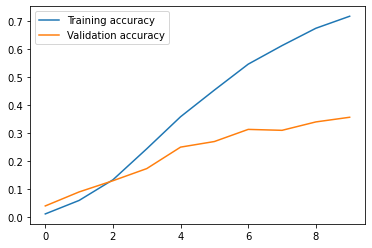
\includegraphics[width=\textwidth]{3-2-antes-2.png}
 		\caption{Valor de precisión en el conjunto de entrenamiento y validación entrenando unicamente el nuevo modelo añadido.}
\end{figure}



En el conjunto de test conseguimos el siguiente valor de precisión:

\begin{lstlisting}
Accuracy con fine tuning (antes de entrenar todo el modelo): 0.3033300362677217
\end{lstlisting}


Y tras hacer toda la red entrenable y reentrenarla, obtenemos el siguiente resultado:


\begin{figure}[H]
  \centering
      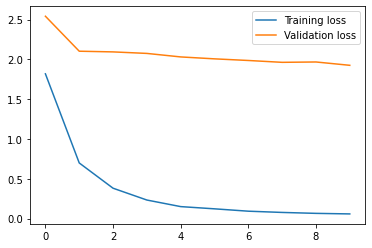
\includegraphics[width=\textwidth]{3-2-1.png}
		\caption{Perdida en el conjunto de entrenamiento y validación entrenando todo el modelo (ResNet50 y capas añadidas).}
\end{figure}

\begin{figure}[H]
  \centering
      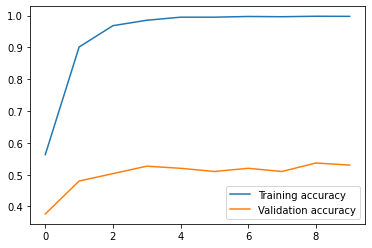
\includegraphics[width=\textwidth]{3-2-2.png}
		\caption{Valor de precisión en el conjunto de entrenamiento y validación entrenando todo el modelo (ResNet50 y capas añadidas).}
\end{figure}



En el conjunto de test conseguimos el siguiente valor de precisión:

\begin{lstlisting}
Accuracy con fine tuning: 0.4701615562149687
\end{lstlisting}

Vemos como la mejora es sustancial, obteniendo el mejor valor de todas las pruebas con ResNet50, como nos confirmaban las distintas fuentes utilizadas.







\newpage

\section{Bonus: Propuestas de mejora de BaseNet}

De cara a realizar el bonus, tras buscar y estudiar el conjunto de datos sobre el que trabajamos\cite{cifar100bonus}, CIFAR100, las mejoras propuestas son las siguientes:

\begin{enumerate}
	\item Uso de activaciones Elu en lugar de ReLu: Con el uso de activaciones ELU en lugar de ReLu, si el valor es menor cero usaremos un valor pequeño negativo, en lugar de anular dicho valor, de forma que sigue aportortando algo a la red, aunque sea pequeño. Se usa un valor reducido en caso de que afecte negativamente a la red, pero permite que valores que si mejorarían la red se utilicen.
	\item Adam\cite{adam} como optimizador: Aunque hemos conseguido buenos resultados con SGD, de forma empírica he comprobado que utilizar este optimizador mejora el resultado.
	\item Uso de máscaras pequeñas en las convoluciones 2D\cite{convksize}.
	\item Cambiado disposición del modelo: Tras buscar referencias y bibliografía\cite{cifar100bonus}, he encontrado que una buena forma de conseguir buenos resultados en reconocimiento de imágenes es que en la red neuronal se vayan aplicando capas de convoluciones 2D con mayor dimensionalidad de salida (en nuestro caso, con sus respectivas activaciones ELU y capas de BatchNormalization), y a su vez se van intercalando capas de MaxPooling para reducir el tamaño de la entrada y manteniendo los valores altos. Finalmente, se aplanará utilizando la capa Flatten, y a partir de ahí aplicaremos capas FC, tantas como convoluciones se hayan realizado.
\end{enumerate}





\begin{figure}[H]
  \centering
      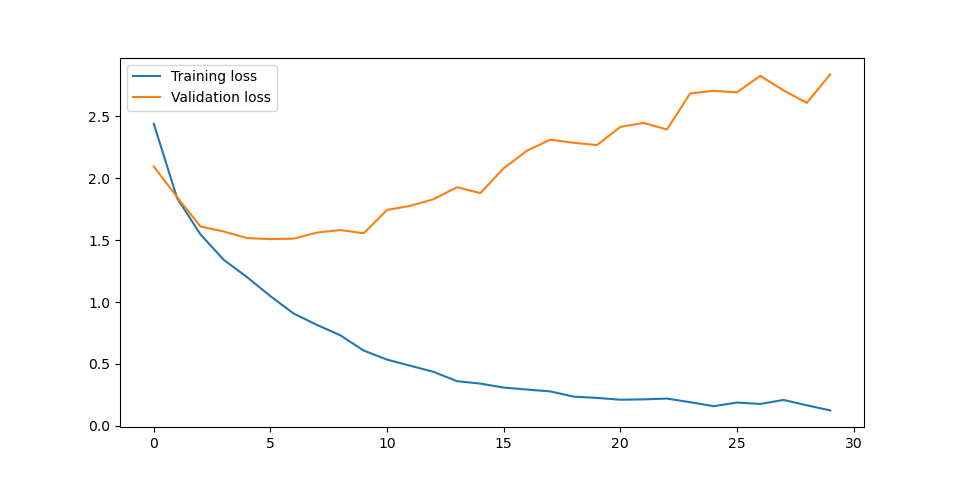
\includegraphics[width=\textwidth]{bonus.png}
		\caption{Perdida en el conjunto de entrenamiento y validación con las nuevas mejoras.}
\end{figure}

\begin{figure}[H]
  \centering
		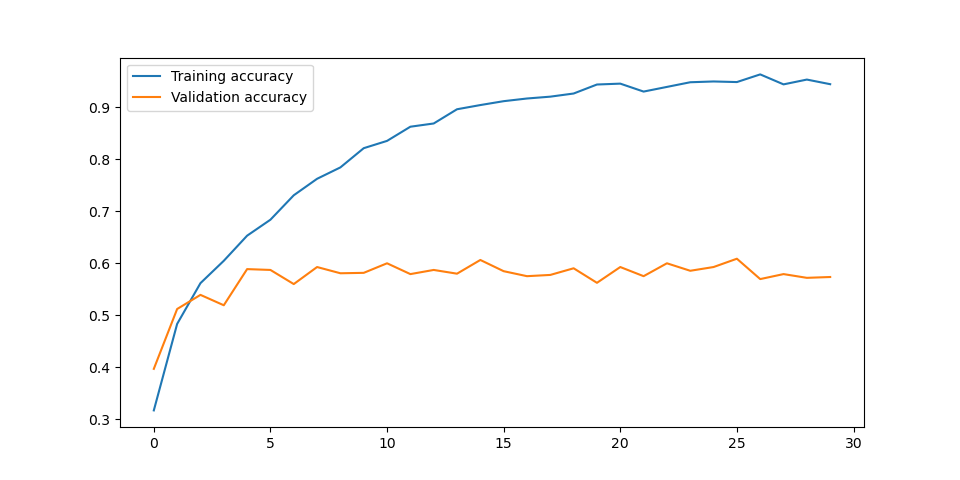
\includegraphics[width=\textwidth]{bonus-1.png}
		\caption{Valor de precisión en el conjunto de entrenamiento y validación con las nuevas mejoras.}
\end{figure}



En el conjunto de test conseguimos el siguiente valor de precisión:

\begin{lstlisting}
Accuracy en el conjunto test con normalizacion, aumento, batch normalization, elu, optimizador Adam y nuevo modelo: 0.6008
\end{lstlisting}

Vemos que conseguimos una mejora sustancial del 10\% del modelo tras todas las mejoras del apartado 2. Como vemos, en este caso ha sido crucial las operaciones de convoluciones seguidas de operaciones de pooling, y no he podido seguir la misma dinámica parra hacer la red más profunda debido a que el tamaño de la entrada no lo permitia y con la operación \texttt{UpSampling2D} no me ha ofrecido buenos resultados, sin embargo con imágenes de mayor tamaño se podría aumentar la profundidad de la red y mejorando su rendimiento.




\newpage

\section{Referencias, material y documentación usada}


\begin{thebibliography}{9}

\bibitem{sequential}
	Clase Sequential - Documentación de Keras

	\url{https://keras.io/api/models/sequential/}


\bibitem{model}

	Clase Model - Documentación de Keras

	\url{https://keras.io/api/models/model/}

\bibitem{conv2d}

	Capa Conv2D - Documentación de Keras

	\url{https://keras.io/api/layers/convolution_layers/convolution2d/}


\bibitem{activation}

	Capa Activation - Documentación de Keras

	\url{https://keras.io/api/layers/core_layers/activation/}

\bibitem{relu}

	Capa ReLu - Documentación de Keras

	\url{https://keras.io/api/layers/activation_layers/relu/}

\bibitem{maxpooling2d}

	Capa MaxPooling2D - Documentación de Keras

	\url{https://keras.io/api/layers/pooling_layers/max_pooling2d/}

\bibitem{softmax}

	Capa Softmax - Documentación de Keras

	\url{https://keras.io/api/layers/activation_layers/softmax/}

\bibitem{dense}

	Capa Dense - Documentación de Keras

	\url{https://keras.io/api/layers/activations/}

\bibitem{flatten}

	Capa Flatten - Documentación de Keras

	\url{https://keras.io/api/layers/reshaping_layers/flatten/}

\bibitem{sgd}

	Optimizador SGD - Documentación de Keras

	\url{https://keras.io/api/optimizers/sgd/}

\bibitem{imagedatagenerator}

	Clase ImageDataGenrator - Documentación de Keras

	\url{https://keras.io/api/preprocessing/image/#imagedatagenerator-class}


\bibitem{batchnormalization}

	Capa BatchNormalization - Documentación de Keras

	\url{https://keras.io/api/layers/normalization_layers/batch_normalization/}


\bibitem{renorm}

	Batch Renormalization: Towards Reducing Minibatch Dependence in Batch-Normalized Models - Sergey Ioffe, 2017

	\url{https://arxiv.org/abs/1702.03275}


\bibitem{dropout}

	Capa Dropout - Documentación de Keras

	\url{https://keras.io/api/layers/regularization_layers/dropout/}


\bibitem{cub200}

	Caltech-UCSD Birds-200

	\url{http://www.vision.caltech.edu/visipedia/CUB-200.html}

\bibitem{resnet50}

	ResNet50 - Documentación de Keras

	\url{https://keras.io/api/applications/resnet/#resnet50-function}


\bibitem{cifar100bonus}

	Best Practices for Convolutional Neural NetworksApplied to Object Recognition in Images - Anderson de Andrade

	\url{https://arxiv.org/pdf/1910.13029.pdf}


\bibitem{finetuningkeras}

	Fine Tuning y congelamiento de capas - Documentación de Keras

	\url{https://keras.io/guides/transfer_learning/}


\bibitem{finetuning}

	Fine-tuning CNN Image Retrievalwith No Human Annotation - Filip Radenovi, Giorgos Tolias, Ondˇrej Chum

	\url{https://arxiv.org/pdf/1711.02512.pdf}


\bibitem{adam}

	Optimizador Adam - Documentación de Keras

	\url{https://keras.io/api/optimizers/adam/}


\bibitem{convksize}

	Very Deep Convolutional Networks for Large-Scale Image Recognition - Karen Simonyan \& Andrew Zisserman

	\url{https://arxiv.org/pdf/1409.1556.pdf}

\end{thebibliography}

\end{document}
